\documentclass[11pt,a4paper]{article}

\usepackage[utf8]{inputenc}
\usepackage[T1]{fontenc}
\usepackage[spanish,es-tabla,es-nodecimaldot]{babel}
\usepackage{lmodern}
\usepackage[margin=2.5cm]{geometry}
\usepackage{amsmath}
\usepackage{graphicx}
\usepackage{booktabs}
\usepackage{array}
\usepackage{float}
\usepackage{subcaption}
\usepackage{tikz}
\usetikzlibrary{positioning,arrows.meta,fit}
\usepackage[authoryear,round]{natbib}
\usepackage{hyperref}
\hypersetup{colorlinks=true,linkcolor=black,citecolor=black,urlcolor=blue}

\graphicspath{{figuras/}}
\setlength{\emergencystretch}{3em}

% Todas las citas del informe van en negrita
\AtBeginDocument{%
  \let\citepOriginal\citep
  \renewcommand*{\citep}[1]{\textbf{\citepOriginal{#1}}}%
  \let\citetOriginal\citet
  \renewcommand*{\citet}[1]{\textbf{\citetOriginal{#1}}}%
  \let\citealpOriginal\citealp
  \renewcommand*{\citealp}[1]{\textbf{\citealpOriginal{#1}}}%
}

\begin{document}

\begin{titlepage}
\centering
{\large Universidad Nacional de Costa Rica\par}
{\large Escuela de Informática\par}
{\large EIF420O Inteligencia Artificial\par}
\vspace{4cm}
{\LARGE\bfseries Laboratorio 02\par}
\vspace{0.5cm}
{\Large Métodos supervisados: clasificación con KNN, Árboles de Decisión, Random Forest, XGBoost y AdaBoost\par}
\vspace{4cm}
{\large Brandon Brenes Umaña -- 119180779\par}
{\large Sebastián Alpízar Porras -- 118240079\par}
{\large Darío Gutiérrez Jiménez -- 119360478\par}
\vspace{2cm}
{\large Profesor: Dr. Juan Murillo-Morera\par}
\vfill
{\large II Ciclo 2026\par}
\end{titlepage}

\tableofcontents
\newpage

% ======================================================================
\section{Introducción}

En el Laboratorio 01 trabajamos con métodos no supervisados, donde no hay una variable de respuesta. En este laboratorio pasamos a la otra rama del framework: los métodos supervisados, y en particular la \textit{clasificación}, en la que el modelo aprende a partir de ejemplos ya etiquetados para predecir la clase de individuos nuevos \citep{hastie2009,james2013}.

Trabajamos con los dos conjuntos de datos que dio el profesor. El primero es \textbf{Potabilidad del agua}: 3276 muestras con 9 mediciones fisicoquímicas, y hay que predecir si el agua es apta para el consumo humano. Las guías de la Organización Mundial de la Salud usan este tipo de parámetros para evaluar la calidad del agua \citep{who2022}. El segundo es \textbf{Predicción de diabetes}: 100\,000 pacientes con datos clínicos y demográficos (edad, índice de masa corporal, hemoglobina glicosilada, glucosa, etc.), y hay que predecir si el paciente tiene diabetes. Dos de esas variables, la HbA1c y la glucosa, son justamente los criterios de diagnóstico que usa la Asociación Americana de Diabetes \citep{ada2024}.

Para cada uno de los cinco algoritmos pedidos (KNN, Árboles de Decisión, Random Forest, XGBoost y AdaBoost) corrimos la configuración estándar y varias variaciones, escogimos el mejor modelo de cada algoritmo y lo analizamos con la matriz de confusión, la importancia de variables y validación cruzada. Al final comparamos los cinco mejores modelos de cada conjunto de datos. Los dos conjuntos son muy distintos: en potabilidad las clases casi no se pueden separar, mientras que en diabetes dos variables bastan para identificar a la mayoría de los diabéticos. Esto nos permitió ver cuándo ayuda y cuándo no ayuda escoger un algoritmo más complejo. Todo se hizo con el framework que hemos construido en el curso, ahora con la rama \texttt{Supervisado} y la clase \texttt{Clasificacion} \citep{pedregosa2011}.

% ======================================================================
\section{Definiciones y conceptos}

\subsection{Aprendizaje supervisado y clasificación}
En el aprendizaje supervisado se tiene un conjunto de individuos descritos por variables predictoras $X$ y una variable a predecir $Y$ que ya se conoce. El objetivo es aprender una función $\hat f$ tal que $\hat f(X)\approx Y$ y que funcione bien con datos que el modelo no vio durante el entrenamiento \citep{james2013}. Cuando $Y$ es categórica se habla de \textit{clasificación}, y cuando es numérica, de regresión. En los dos datasets de este laboratorio $Y$ es binaria (0 o 1). Para medir qué tan bien generaliza el modelo, los datos se dividen en un conjunto de entrenamiento, con el que se ajusta el modelo, y uno de prueba, con el que se evalúa \citep{hastie2009}.

\subsection{K vecinos más cercanos (KNN)}
KNN clasifica un individuo nuevo buscando los $k$ individuos de entrenamiento más cercanos y asignándole la clase que más se repite entre ellos \citep{cover1967}. No construye un modelo explícito: guarda los datos y calcula distancias en el momento de predecir. La distancia más usada es la de Minkowski,
\[
d(x,z)=\Big(\sum_{j=1}^{p}|x_j-z_j|^{q}\Big)^{1/q},
\]
que con $q=2$ es la euclídea y con $q=1$ la de Manhattan. Los parámetros principales son $k$, el tipo de distancia y los pesos: con pesos uniformes todos los vecinos votan igual, y con pesos por distancia los más cercanos pesan más. Un $k$ pequeño da fronteras muy irregulares (sobreajuste), y uno grande las suaviza demasiado. Como KNN depende de las distancias, las variables se deben estandarizar. Si no, las que tienen valores más grandes dominan el cálculo \citep{james2013}.

\subsection{Árboles de Decisión (DT)}
Un árbol de decisión divide los datos con preguntas sucesivas del tipo ``¿$x_j\le c$?'' hasta llegar a hojas que asignan una clase \citep{breiman1984,quinlan1986}. En cada nodo se escoge la división que más reduce la impureza. Las medidas más comunes son el índice de Gini y la entropía:
\[
G=1-\sum_{c}p_c^{2},\qquad H=-\sum_{c}p_c\log_2 p_c ,
\]
donde $p_c$ es la proporción de la clase $c$ en el nodo. Si no se limita, el árbol crece hasta que cada hoja es pura y memoriza el conjunto de entrenamiento. Por eso se controla con la profundidad máxima (\texttt{max\_depth}), el mínimo de individuos por hoja (\texttt{min\_samples\_leaf}) o la poda por costo-complejidad (\texttt{ccp\_alpha}) \citep{breiman1984}. Su ventaja principal es que se puede interpretar: las reglas del árbol se leen directamente.

\subsection{Random Forest (RF)}
Random Forest es un ensamble de muchos árboles de decisión \citep{breiman2001}. Cada árbol se entrena con una muestra bootstrap de los datos (\textit{bagging}, \citealp{breiman1996}), y en cada división solo se considera un subconjunto aleatorio de variables (\texttt{max\_features}, por defecto $\sqrt{p}$). La predicción final es el voto de todos los árboles. El muestreo de variables hace que los árboles se parezcan menos entre sí, y al promediar árboles poco correlacionados la varianza baja mucho sin aumentar el sesgo. Por eso RF suele ser mucho más estable que un solo árbol \citep{hastie2009}.

\subsection{AdaBoost}
AdaBoost (\textit{Adaptive Boosting}) también combina muchos clasificadores débiles, pero los entrena en secuencia \citep{freund1997}. Empieza con todos los individuos con el mismo peso. Después de cada clasificador, aumenta el peso de los individuos mal clasificados para que el siguiente se concentre en ellos. Cada clasificador $h_m$ recibe un peso $\alpha_m=\eta\,\tfrac12\ln\!\big(\tfrac{1-\varepsilon_m}{\varepsilon_m}\big)$ según su error $\varepsilon_m$, y la predicción es el voto ponderado $\operatorname{signo}\big(\sum_m\alpha_m h_m(x)\big)$. El clasificador débil por defecto es un árbol de profundidad 1 (\textit{stump}), y $\eta$ es la tasa de aprendizaje.

\subsection{XGBoost}
XGBoost (\textit{eXtreme Gradient Boosting}) es una implementación optimizada del \textit{gradient boosting} \citep{friedman2001,chen2016}. Cada árbol nuevo se ajusta al gradiente de la función de pérdida de los árboles anteriores, o sea, corrige los errores que quedan. Además, la función objetivo agrega una penalización por la complejidad de los árboles:
\[
\mathcal{L}=\sum_i \ell(y_i,\hat y_i)+\sum_m\Big(\gamma T_m+\tfrac12\lambda\lVert w_m\rVert^2\Big),
\]
donde $T_m$ es la cantidad de hojas y $w_m$ los pesos de las hojas del árbol $m$ \citep{chen2016}. Los parámetros principales son la cantidad de árboles (\texttt{n\_estimators}), la tasa de aprendizaje (\texttt{learning\_rate}), la profundidad (\texttt{max\_depth}), las proporciones de filas y columnas que usa cada árbol (\texttt{subsample}, \texttt{colsample\_bytree}) y \texttt{scale\_pos\_weight}, que le da más peso a la clase positiva cuando las clases están desbalanceadas.

\subsection{Preprocesamiento y selección de atributos}
Antes de entrenar hay que preparar los datos. Los valores faltantes se \textit{imputan} (con la mediana o la media), las variables numéricas se \textit{estandarizan} para los métodos basados en distancias y las categóricas se transforman con \textit{one-hot}, o sea, una columna 0/1 por categoría \citep{james2013}. Todo eso se debe calcular solo con el conjunto de entrenamiento. Si se usan los datos de prueba, por ejemplo para calcular la mediana, hay fuga de información y los resultados salen optimistas \citep{hastie2009}. La \textit{selección de atributos} se queda con las variables más útiles. Nosotros usamos \texttt{SelectKBest} con el estadístico $F$ del ANOVA, que ordena las variables según qué tanto cambia su media entre clases \citep{guyon2003}.

\subsection{Índices de calidad}
Con la matriz de confusión (filas = clase real, columnas = predicción), y tomando la clase 1 como positiva, se obtienen los verdaderos positivos (VP), verdaderos negativos (VN), falsos positivos (FP) y falsos negativos (FN) \citep{sokolova2009}. Con ellos se calculan:
\begin{itemize}
  \item \textbf{Precisión global (PG)}: $(VP+VN)/n$, y el error global $EG=1-PG$.
  \item \textbf{Precisión por clase}: los aciertos de cada clase entre el total real de esa clase. Para la clase 1 es el \textbf{Recall} o sensibilidad, $VP/(VP+FN)$, y para la clase 0 es la especificidad.
  \item \textbf{Precision o valor predictivo positivo (VPP)}: $VP/(VP+FP)$, de los que el modelo dice que son positivos, cuántos lo son.
  \item \textbf{F1}: la media armónica de VPP y Recall, $2\cdot\mathrm{VPP}\cdot\mathrm{Recall}/(\mathrm{VPP}+\mathrm{Recall})$.
  \item \textbf{F1 macro}: el promedio del F1 de las dos clases, de modo que las dos pesan igual sin importar su tamaño.
  \item \textbf{AUC}: el área bajo la curva ROC, que grafica la tasa de verdaderos positivos contra la de falsos positivos para todos los umbrales posibles. Es la probabilidad de que el modelo le dé más puntaje a un positivo que a un negativo escogidos al azar \citep{fawcett2006}.
\end{itemize}
Cuando las clases están desbalanceadas, la PG engaña. Un modelo que dice que nadie tiene diabetes acierta el 91\,\% en nuestros datos, pero no sirve para nada \citep{he2009}. Por eso usamos el \textbf{F1 macro} como criterio para escoger el mejor modelo de cada algoritmo, y la AUC como apoyo.

\subsection{Validación cruzada}
Un solo conjunto de prueba puede dar un resultado con suerte. En la validación cruzada con $K$ particiones, el conjunto de entrenamiento se divide en $K$ partes, se entrena con $K-1$ y se evalúa con la restante, y se repite $K$ veces \citep{kohavi1995}. El promedio estima el desempeño y la desviación estándar indica qué tan estable es. Usamos $K=5$ estratificada, es decir, cada parte mantiene la proporción de clases.

% ======================================================================
\section{Mapa conceptual}

El mapa resume cómo se relacionan los conceptos del curso hasta ahora. Siguiendo a \citet{james2013}, el aprendizaje automático se divide en métodos no supervisados, donde no hay una variable a predecir y se buscan estructuras en los datos, y métodos supervisados, donde se aprende a predecir una variable a partir de las demás. La parte superior es el mapa conceptual del primer laboratorio (métodos no supervisados) y la parte inferior agrega los métodos de clasificación de este laboratorio. Estos se organizan como en \citet{hastie2009}: métodos basados en instancias, árboles y ensambles por \textit{bagging} o \textit{boosting}, todos con el mismo preprocesamiento y los mismos índices de evaluación. El EDA es común a los dos laboratorios.

\begin{figure}[H]
\centering
\resizebox{\textwidth}{!}{%
\begin{tikzpicture}[
  every node/.style={draw,rounded corners,align=center,font=\small},
  n0/.style={fill=gray!40,font=\Large\bfseries},
  n1/.style={fill=gray!20,font=\bfseries},
  n2/.style={fill=blue!10},
  n3/.style={fill=orange!15},
  n4/.style={draw=gray,font=\footnotesize,text width=3.4cm},
  n5/.style={fill=green!10,text width=12.5cm},
  et/.style={draw=none,font=\itshape\small,text=gray},
  -{Stealth},thick]
% ---------------- Raíz común ----------------
\node[n0] (raiz) {Aprendizaje automático};
\node[n2,above=0.6cm of raiz] (eda) {EDA: nulos, duplicados, outliers, correlación, estandarizar};
\draw (eda) -- (raiz);
% ---------------- Laboratorio 1: métodos no supervisados ----------------
\node[n1,below=1cm of raiz] (ns) {Métodos no supervisados};
\node[n2,below left=0.8cm and 3.5cm of ns] (red) {Reducción de dimensionalidad};
\node[n2,below right=0.8cm and 3.5cm of ns] (clu) {Clustering};
\node[n3,below left=0.8cm and -0.3cm of red] (acp) {ACP (lineal)};
\node[n3,below right=0.8cm and -0.3cm of red] (nl) {t-SNE y UMAP\\(no lineales)};
\node[n3,below left=0.8cm and -0.3cm of clu] (hac) {HAC (jerárquico)};
\node[n3,below right=0.8cm and -0.3cm of clu] (km) {K-means (centroides)};
\node[n4,below=0.5cm of acp] (b1) {autovalores y autovectores; varianza explicada; círculo de correlación; plano principal};
\node[n4,below=0.5cm of nl] (b2) {t-SNE: perplexity, KL\\UMAP: n\_neighbors, min\_dist\\sirven para visualizar};
\node[n4,below=0.5cm of hac] (b3) {enlace simple, completo, promedio, Ward; dendrograma; silhouette};
\node[n4,below=0.5cm of km] (b4) {escoger $k$; inercia; método del codo; k-means++; silhouette};
\node[et,right=0.3cm of ns] {(Laboratorio 1)};
\draw (raiz) -- (ns);
\draw (ns) -- (red); \draw (ns) -- (clu);
\draw (red) -- (acp); \draw (red) -- (nl);
\draw (clu) -- (hac); \draw (clu) -- (km);
\draw (acp) -- (b1); \draw (nl) -- (b2); \draw (hac) -- (b3); \draw (km) -- (b4);
\draw[dashed,blue] (acp.east) to[bend left=14] node[draw=none,pos=0.62,above,font=\scriptsize]{las componentes se usan como entrada} (hac.west);
% ---------------- Laboratorio 2: métodos supervisados ----------------
\path (ns |- b1.south) ++(0,-1.6) node[n1] (sup) {Métodos supervisados};
\node[et,left=0.3cm of sup] {(Laboratorio 2)};
\draw (raiz.east) -- ++(10.2,0) |- (sup.east);
\node[n1,below=3.1cm of sup] (cl) {Clasificación supervisada\\(variable a predecir categórica)};
\node[n5,above=0.7cm of cl] (pre) {\textbf{Preparación}: partición entrenamiento/prueba estratificada; imputación (mediana); estandarización (KNN); one-hot de categóricas; selección de atributos (\texttt{SelectKBest}); todo dentro de un \texttt{Pipeline} para evitar fuga de información};
\node[n2,below left=1cm and 3.2cm of cl] (ins) {Basado en instancias};
\node[n2,below=1cm of cl] (arb) {Un solo árbol};
\node[n2,below right=1cm and 3.2cm of cl] (ens) {Ensambles de árboles};
\node[n3,below=0.6cm of ins] (knn) {KNN};
\node[n3,below=0.6cm of arb] (dt) {Árbol de Decisión};
\node[n3,below left=0.6cm and -0.6cm of ens] (rf) {Random Forest\\(\textit{bagging})};
\node[n3,below right=0.6cm and -0.6cm of ens] (bo) {AdaBoost y XGBoost\\(\textit{boosting})};
\node[n4,below=0.5cm of knn] (a1) {$k$, distancia (euclídea, Manhattan), pesos; necesita escalar};
\node[n4,below=0.5cm of dt] (a2) {Gini o entropía; profundidad, mínimo por hoja, poda; reglas interpretables};
\node[n4,below=0.5cm of rf] (a3) {muestras bootstrap + variables al azar; voto de muchos árboles; baja la varianza};
\node[n4,below=0.5cm of bo] (a4) {árboles en secuencia que corrigen errores; tasa de aprendizaje; \texttt{scale\_pos\_weight}};
\node[n5,below=4.4cm of arb] (ev) {\textbf{Evaluación}: matriz de confusión; PG y EG; precisión por clase (Recall); VPP; F1 y \textbf{F1 macro} (criterio de selección); curva ROC y AUC; validación cruzada estratificada; importancia de variables};
\draw (sup) -- (pre);
\draw (pre) -- (cl);
\draw (cl) -- (ins); \draw (cl) -- (arb); \draw (cl) -- (ens);
\draw (ins) -- (knn); \draw (arb) -- (dt); \draw (ens) -- (rf); \draw (ens) -- (bo);
\draw (knn) -- (a1); \draw (dt) -- (a2); \draw (rf) -- (a3); \draw (bo) -- (a4);
\draw (a1) -- (ev); \draw (a2) -- (ev); \draw (a3) -- (ev); \draw (a4) -- (ev);
\draw[dashed,blue] (dt.east) to[bend left=12] node[draw=none,above,font=\scriptsize]{es el clasificador base} (ens.west);
\end{tikzpicture}}
\caption{Mapa conceptual del curso: métodos no supervisados del primer laboratorio (arriba) y métodos de clasificación de este laboratorio (abajo).}
\end{figure}

% ======================================================================
\section{Datos y framework utilizado}

\subsection{Conjuntos de datos}
\begin{itemize}
  \item \texttt{water\_potability.csv} \citep{kadiwal2021}: 3276 filas y 10 columnas. Las 9 predictoras son numéricas: \texttt{ph}, \texttt{Hardness}, \texttt{Solids}, \texttt{Chloramines}, \texttt{Sulfate}, \texttt{Conductivity}, \texttt{Organic\_carbon}, \texttt{Trihalomethanes} y \texttt{Turbidity}. La variable a predecir es \texttt{Potability} (1 = potable).
  \item \texttt{diabetes\_prediction\_dataset.csv} \citep{mustafa2023}: 100\,000 filas y 9 columnas. Las predictoras son \texttt{gender} y \texttt{smoking\_history} (categóricas), \texttt{age}, \texttt{hypertension}, \texttt{heart\_disease}, \texttt{bmi}, \texttt{HbA1c\_level} y \texttt{blood\_glucose\_level}. La variable a predecir es \texttt{diabetes} (1 = diabético).
\end{itemize}

\subsection{Framework}
El framework sigue la estructura vista en clase, con la clase base \texttt{EDA} de la que heredan las ramas no supervisada y supervisada. Para este laboratorio agregamos la rama supervisada:
\begin{itemize}
  \item \texttt{Supervisado(EDA)} (carpeta \texttt{supervisado/}): tiene lo que comparten la clasificación y la regresión. Hace la partición entrenamiento/prueba estratificada, arma el \texttt{Pipeline} de preprocesamiento (imputación, escalado, one-hot y \texttt{SelectKBest}), entrena, calcula los índices de calidad, guarda el historial de experimentos y tiene \texttt{validacion\_cruzada}, \texttt{mejor\_modelo}, \texttt{matriz\_confusion} y los gráficos de matriz, ROC y comparación.
  \item \texttt{Clasificacion(Supervisado)} (carpeta \texttt{clasificacion/}): los métodos \texttt{knn}, \texttt{arbol}, \texttt{bosque}, \texttt{xgboost} y \texttt{adaboost}. Llamados sin parámetros, dan la configuración estándar, que son los valores por defecto de las librerías. Los parámetros extra pasan directo al estimador. También tiene \texttt{comparar} (varias configuraciones de una vez), \texttt{curva\_k}, \texttt{importancia\_variables} y \texttt{graficar\_arbol}.
\end{itemize}
Los estimadores son los de scikit-learn \citep{pedregosa2011} y la librería \texttt{xgboost} \citep{chen2016}. Igual que en el Laboratorio 01, se mantiene la estructura MVC. Si se le pasa \texttt{variable\_predecir}, el \texttt{DataFrameModel} crea un objeto \texttt{Clasificacion}, y el \texttt{DataFrameController} recibe acciones como ``\texttt{Comparar}'', ``\texttt{Mejor modelo}'', ``\texttt{Matriz confusión}'', ``\texttt{Validación cruzada}'', ``\texttt{Importancia}'' o ``\texttt{ROC}''. Además, todo el framework quedó en una aplicación web (\texttt{App\_Analitica}, hecha con Streamlit), donde se pueden correr los mismos experimentos con un clic.
\begin{verbatim}
Laboratorio 2/
  clasificacion.ipynb   notebook con todos los experimentos de este informe
  datos/                water_potability.csv, diabetes_prediction_dataset.csv
  eda/                  clase EDA
  no_supervisado/       clase NoSupervisado(EDA)  (Laboratorio 01)
  supervisado/          clase Supervisado(EDA)
  clasificacion/        clase Clasificacion(Supervisado)
  mvc/                  DataFrameModel, DataFrameView, DataFrameController
\end{verbatim}

\subsection{Protocolo experimental}
Usamos el mismo protocolo para los dos datasets, de modo que todas las comparaciones fueran justas \citep{kohavi1995}:
\begin{enumerate}
  \item Se eliminan las filas duplicadas y se hace una partición estratificada de 75\,\% para entrenamiento y 25\,\% para prueba, con semilla 42. Todos los modelos usan \texttt{random\_state=42}, así que el notebook da los mismos resultados cada vez que se corre.
  \item El preprocesamiento va dentro del \texttt{Pipeline}, así que la mediana para imputar, la media y la desviación para escalar y las categorías del one-hot se calculan solo con el entrenamiento.
  \item Para cada algoritmo se corre la configuración estándar y varias variaciones, y se escoge la de mayor \textbf{F1 macro} en el conjunto de prueba.
  \item El mejor modelo de cada algoritmo se analiza con su matriz de confusión, la importancia de variables (en los modelos de árboles) y una validación cruzada estratificada de 5 particiones sobre el entrenamiento, para ver si el resultado es estable.
\end{enumerate}

% ======================================================================
\section{Potabilidad del agua}

\subsection{Análisis exploratorio}
Como recomienda \citet{tukey1977}, antes de modelar revisamos los datos. Todas las variables son numéricas y no hay filas duplicadas, pero hay valores faltantes en \texttt{Sulfate} (781, el 23.8\,\%), \texttt{ph} (491, el 15.0\,\%) y \texttt{Trihalomethanes} (162, el 4.9\,\%). Eliminar esas filas habría dejado solo 2011 de las 3276, así que las imputamos con la mediana dentro del pipeline. Las clases están moderadamente desbalanceadas: 1998 muestras no potables (61.0\,\%) y 1278 potables (39.0\,\%). La partición dejó 2457 filas para entrenamiento y 819 para prueba (499 no potables y 320 potables), con la misma proporción en ambos conjuntos.

\begin{figure}[H]
\centering
\begin{subfigure}{0.52\textwidth}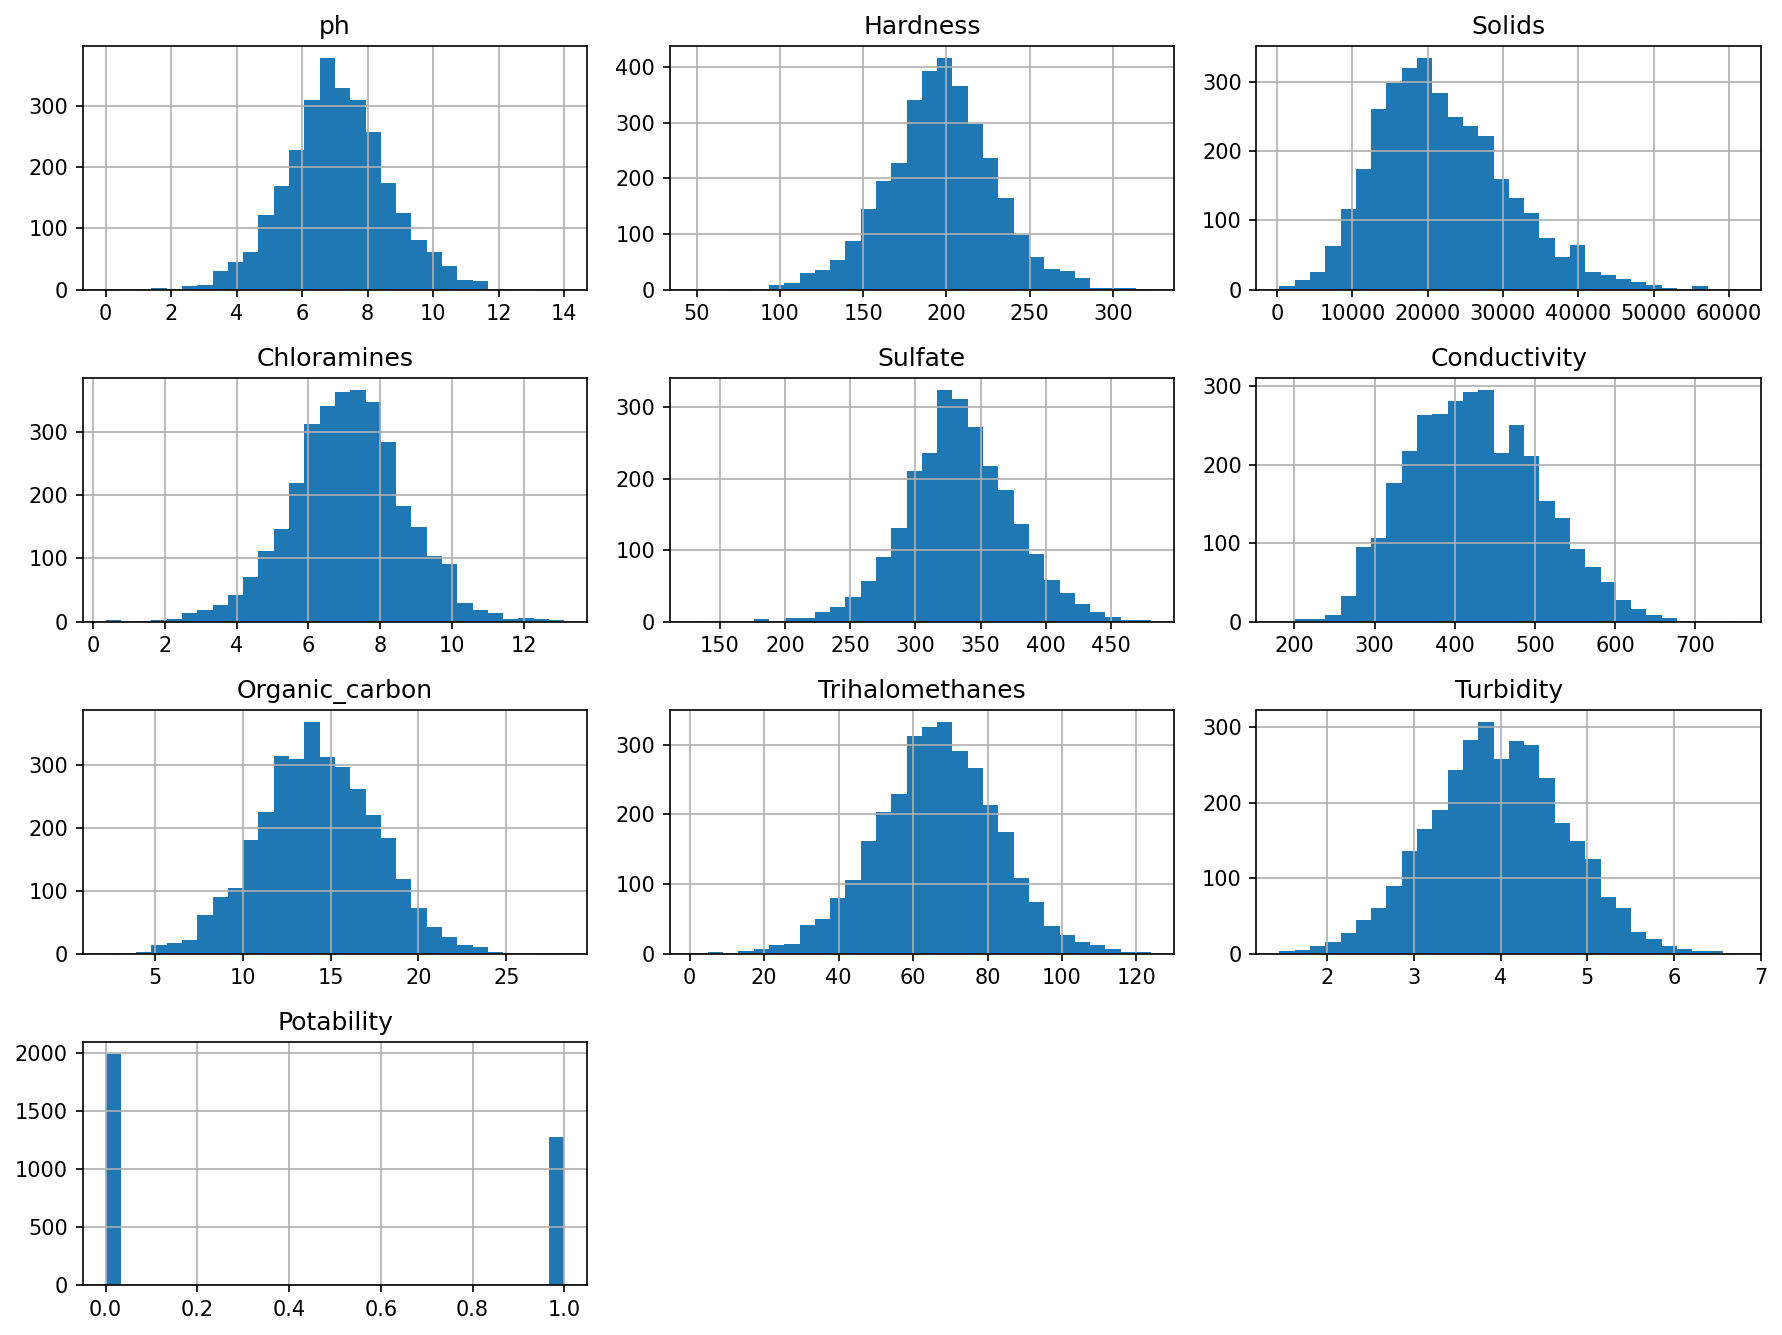
\includegraphics[width=\linewidth]{potabilidad/histogramas.png}\caption{Histogramas}\end{subfigure}
\begin{subfigure}{0.46\textwidth}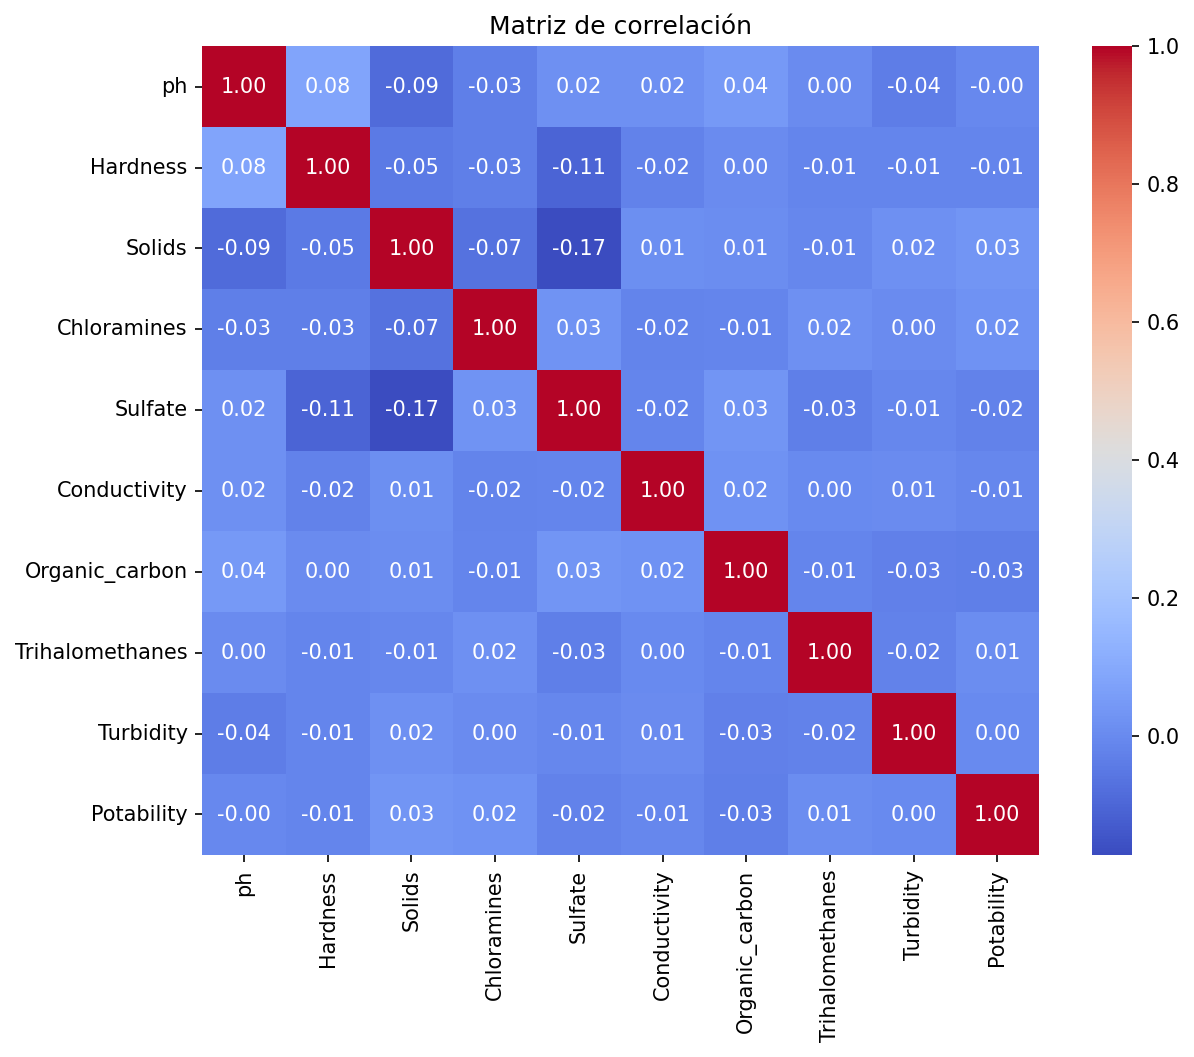
\includegraphics[width=\linewidth]{potabilidad/mapa_calor.png}\caption{Mapa de calor}\end{subfigure}
\caption{Distribución y correlaciones de las variables de potabilidad.}
\end{figure}

Lo más importante del análisis exploratorio es que \textbf{ninguna variable se relaciona linealmente con la potabilidad}. La correlación más alta con \texttt{Potability} es la de \texttt{Solids} ($r=0.034$), y todas están entre $-0.030$ y $0.034$. Las predictoras tampoco se correlacionan entre ellas, y casi todas tienen una distribución parecida a la normal. Los boxplots por clase son casi idénticos. Eso es raro para datos reales: por ejemplo, el promedio de \texttt{Solids} es 22\,014 ppm, mucho más de los 1200 mg/L de sólidos disueltos a partir de los cuales la OMS considera que el agua tiene un sabor inaceptable \citep{who2022}, y aun así el 39\,\% de las muestras está etiquetada como potable. Por eso esperábamos desde el principio que cualquier modelo tendría un desempeño bajo.

\begin{figure}[H]
\centering
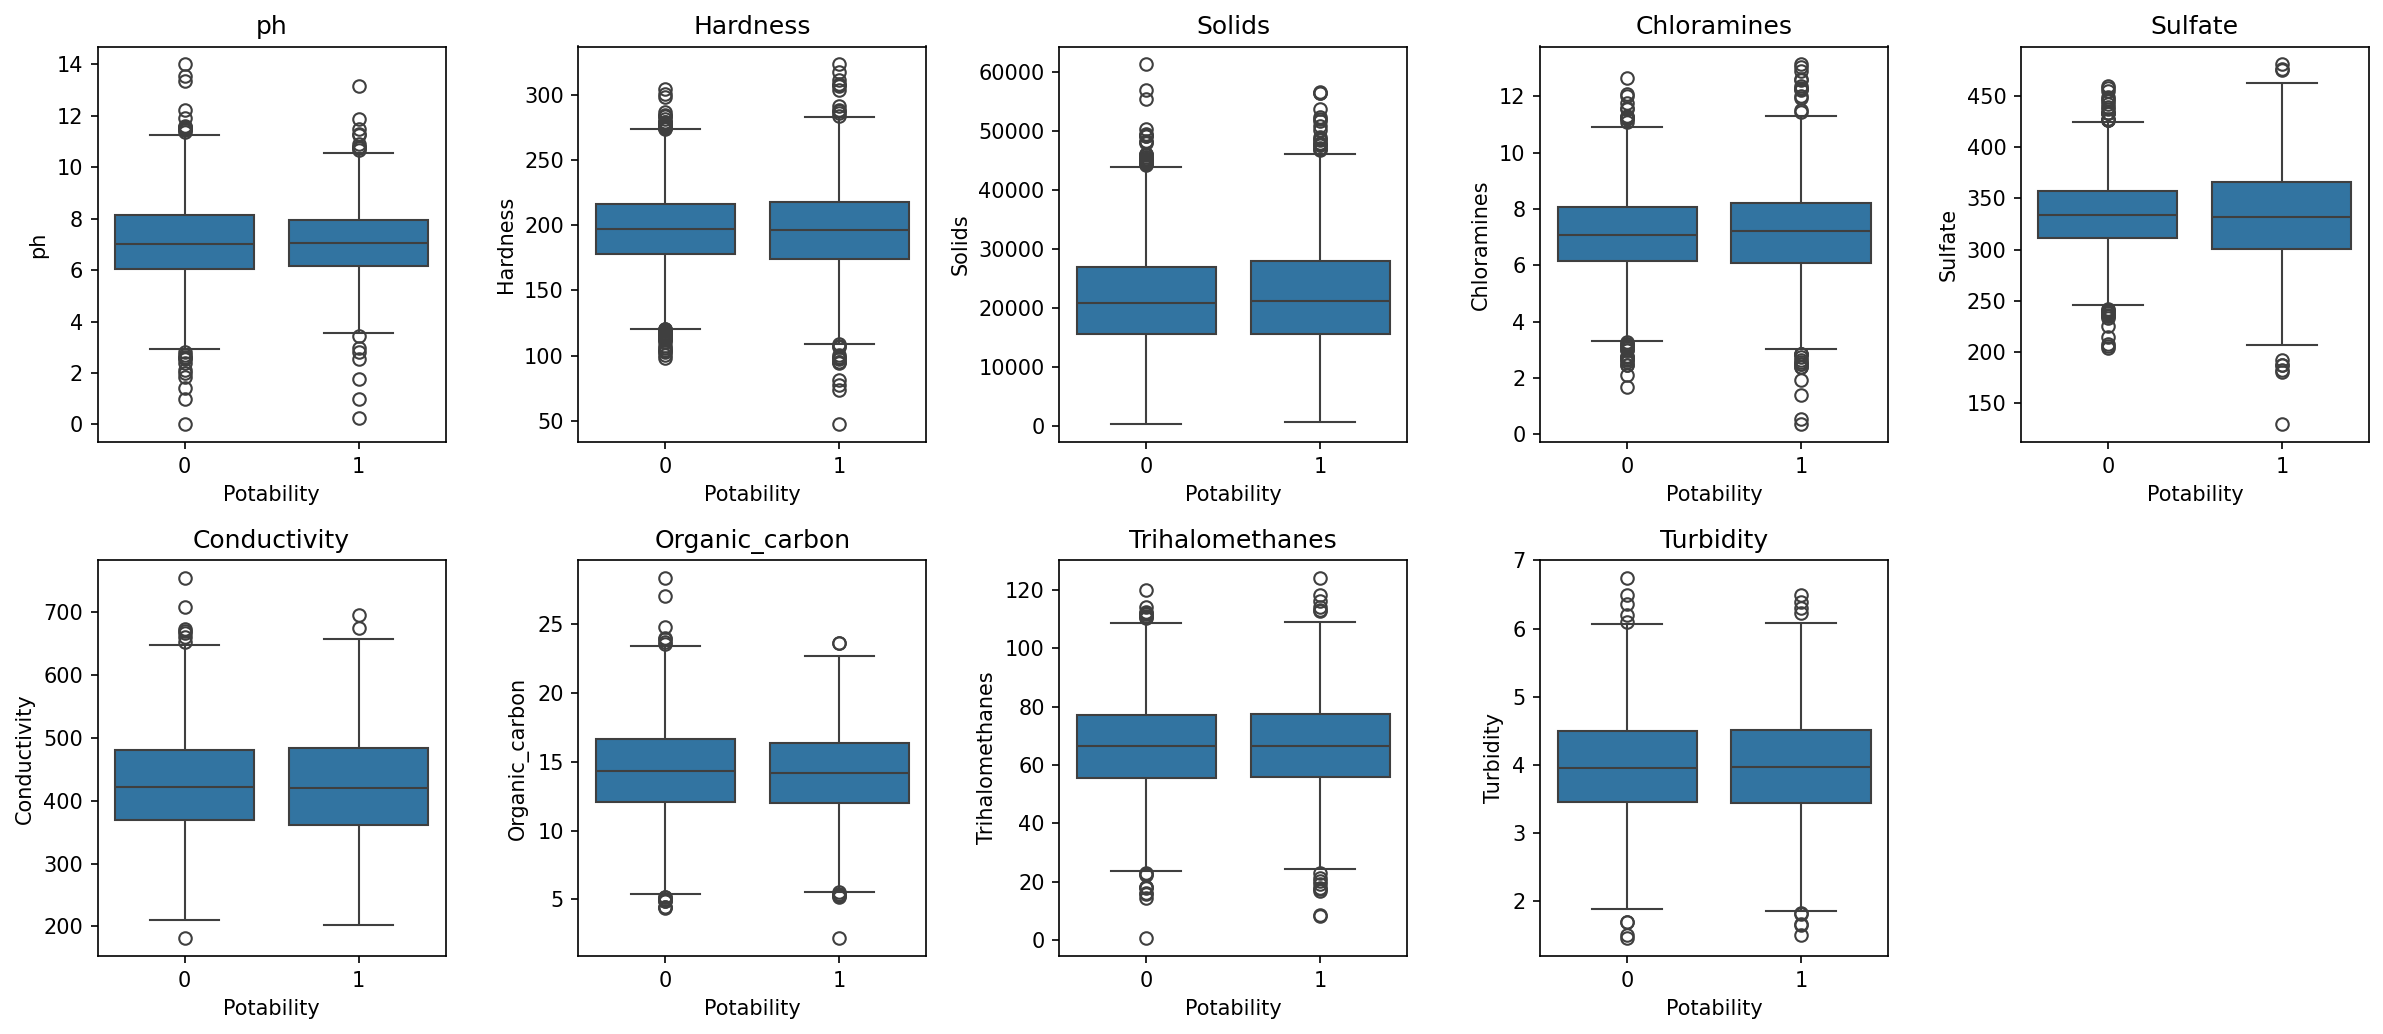
\includegraphics[width=\textwidth]{potabilidad/boxplots_clase.png}
\caption{Distribución de cada variable según la clase (0 = no potable, 1 = potable).}
\end{figure}

El gráfico de radar muestra la media estandarizada de cada una de las 9 variables en cada clase. Todas las diferencias son menores a 0.07 desviaciones estándar. Las más grandes están en \texttt{Solids} ($+0.042$ en las potables contra $-0.027$ en las no potables), \texttt{Organic\_carbon} ($-0.038$ contra $+0.024$), \texttt{Chloramines} y \texttt{Sulfate}. Como explican \citet{he2009}, cuando las clases se traslapan tanto, el problema es de los datos y no del algoritmo.

\begin{figure}[H]
\centering
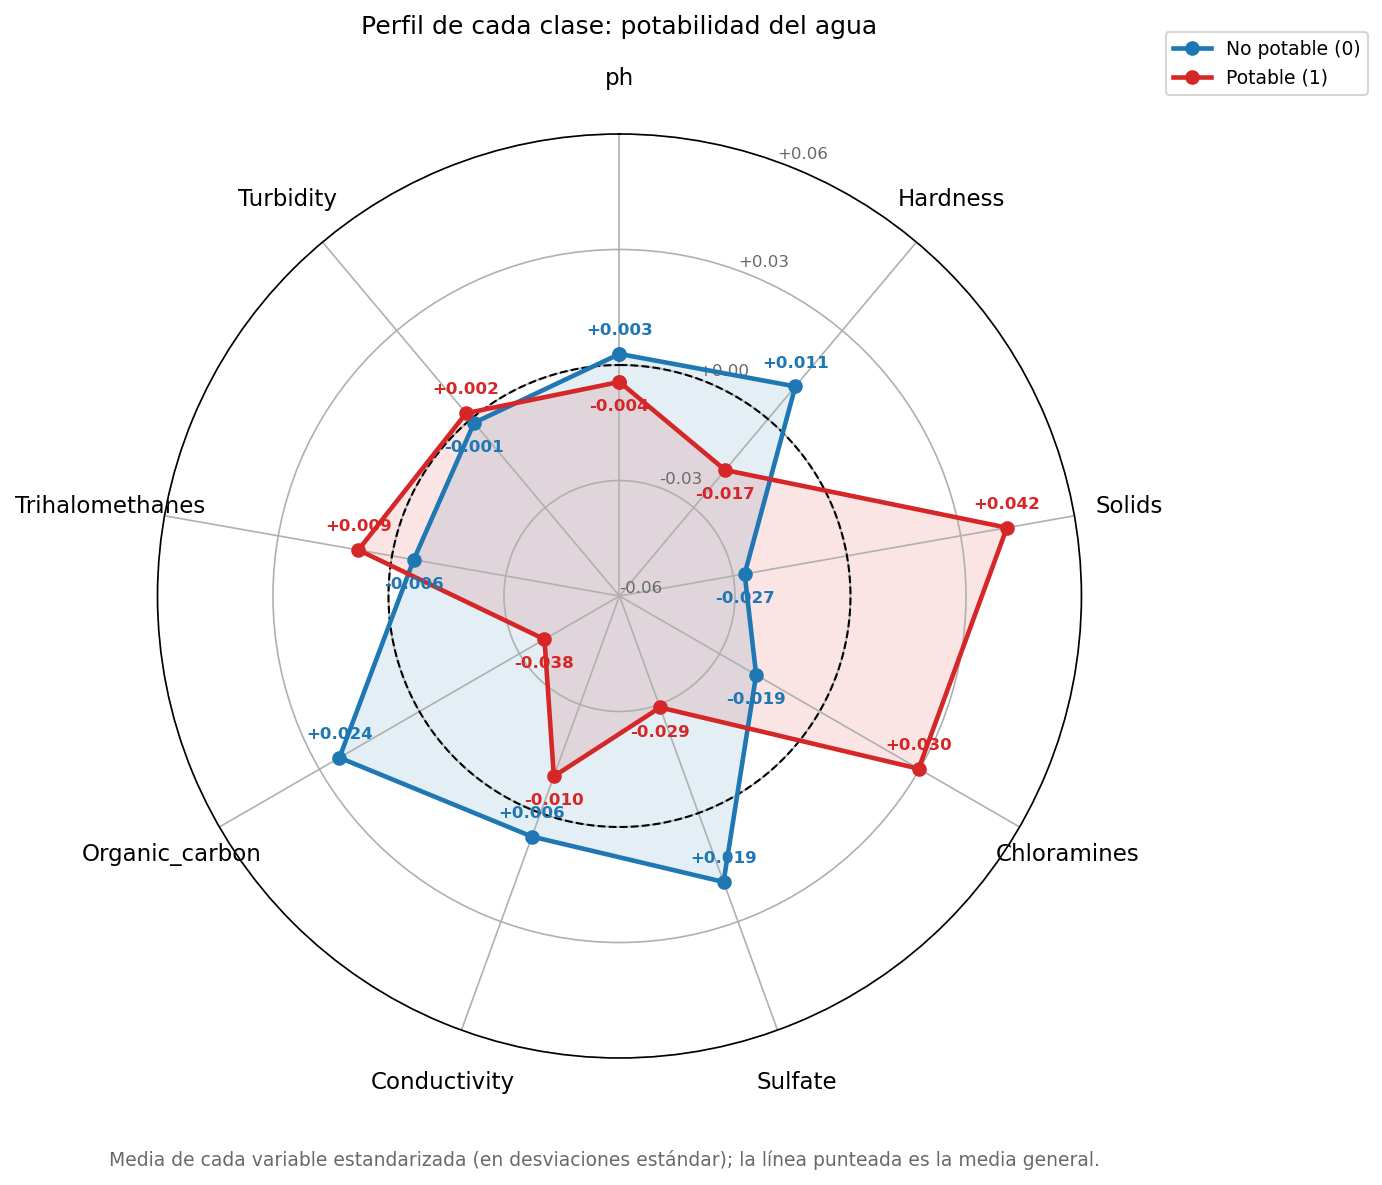
\includegraphics[width=0.72\textwidth]{potabilidad/radar_clases.png}
\caption{Radar con la media estandarizada de las 9 variables en cada clase.}
\end{figure}

Para tener un punto de referencia, un clasificador que diga siempre ``no potable'' tendría en el conjunto de prueba una PG de $499/819=0.6093$, un F1 macro de 0.3786 y una AUC de 0.5. Un modelo solo aporta algo si supera claramente esos valores.

\subsection{KNN}
Siguiendo a \citet{cover1967}, la configuración estándar es la de scikit-learn: $k=5$, pesos uniformes y distancia euclídea, con los datos estandarizados. Como variaciones probamos $k=15$ y $k=25$, pesos por distancia, distancia de Manhattan, imputación con la media, quitar el escalado y quedarse con solo 5 atributos con \texttt{SelectKBest}.

\begin{table}[H]
\centering
\small
\caption{Configuraciones de KNN en potabilidad. La fila en negrita es el mejor modelo según el F1 macro.}
\setlength{\tabcolsep}{4pt}
\begin{tabular}{>{\raggedright\arraybackslash}p{4.9cm}ccccccc}
\toprule
Configuración & PG & Prec.\ 0 & Recall & VPP & F1 & F1 macro & AUC \\
\midrule
\textbf{estándar} & \textbf{0.6093} & \textbf{0.7836} & \textbf{0.3375} & \textbf{0.5000} & \textbf{0.4030} & \textbf{0.5563} & \textbf{0.6037} \\
n\_neighbors=\allowbreak{}15 & 0.6410 & 0.8918 & 0.2500 & 0.5970 & 0.3524 & 0.5521 & 0.6258 \\
n\_neighbors=\allowbreak{}25 & 0.6484 & 0.9299 & 0.2094 & 0.6569 & 0.3175 & 0.5403 & 0.6375 \\
n\_neighbors=\allowbreak{}25, \allowbreak weights=\allowbreak{}distance & 0.6471 & 0.9279 & 0.2094 & 0.6505 & 0.3168 & 0.5395 & 0.6403 \\
n\_neighbors=\allowbreak{}25, \allowbreak p=\allowbreak{}1 & 0.6374 & 0.9218 & 0.1938 & 0.6139 & 0.2945 & 0.5252 & 0.6278 \\
n\_neighbors=\allowbreak{}25, \allowbreak imputación mean & 0.6471 & 0.9319 & 0.2031 & 0.6566 & 0.3103 & 0.5366 & 0.6369 \\
n\_neighbors=\allowbreak{}25, \allowbreak sin escalar & 0.6081 & 0.9299 & 0.1062 & 0.4928 & 0.1748 & 0.4589 & 0.5384 \\
n\_neighbors=\allowbreak{}25, \allowbreak 5 atributos & 0.6239 & 0.8978 & 0.1969 & 0.5526 & 0.2903 & 0.5173 & 0.5901 \\
\bottomrule
\end{tabular}
\end{table}

\begin{figure}[H]
\centering
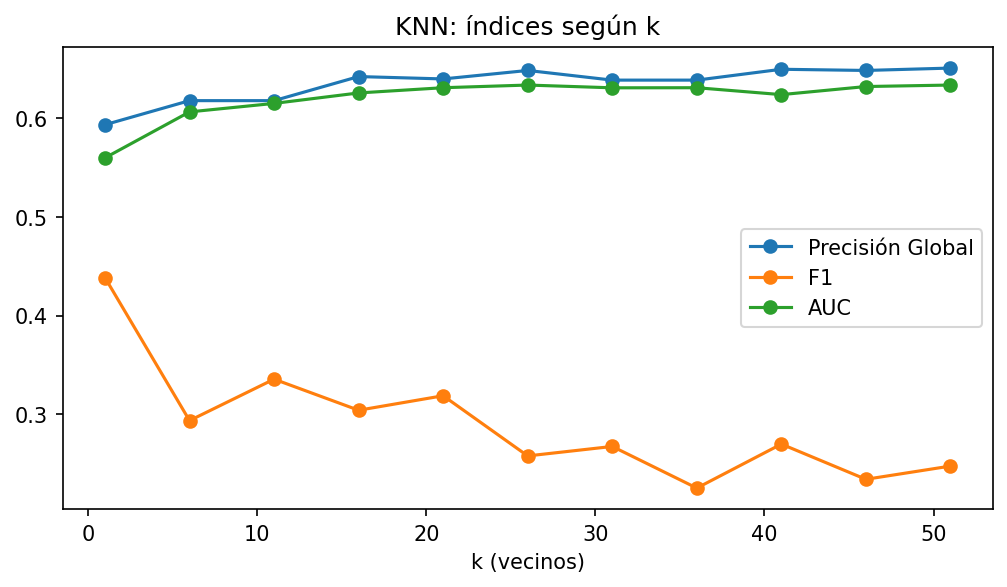
\includegraphics[width=0.7\textwidth]{potabilidad/knn_curva_k.png}
\caption{Índices de KNN según la cantidad de vecinos $k$.}
\end{figure}

La curva de $k$ explica la tabla. Al subir $k$, la PG pasa de 0.593 ($k=1$) a 0.651 ($k=51$), pero el F1 de la clase potable baja de 0.438 a 0.247. Con muchos vecinos, la mayoría casi siempre es ``no potable'', así que el modelo se acerca al clasificador trivial: con $k=25$ la precisión de la clase 0 es 0.93, pero solo detecta el 20.9\,\% de las muestras potables. Por eso el F1 macro escoge la \textbf{configuración estándar ($k=5$)}, que es la que más equilibra las dos clases (F1 macro 0.5563 y Recall 0.3375), aunque su PG (0.6093) es igual a la del clasificador trivial. Escalar es indispensable, tal como dice \citet{james2013}: sin escalar, \texttt{Solids} (con valores de miles) domina la distancia y el F1 macro cae a 0.4589. La selección de atributos empeoró el modelo (0.5173). El ANOVA $F$ ordena las variables según la diferencia de medias entre clases, y en este dataset esa diferencia es casi nula para todas, así que el criterio no tiene con qué escoger \citep{guyon2003}. Los pesos por distancia, la distancia de Manhattan y la imputación con la media casi no cambian nada.

\subsection{Árboles de Decisión}
La configuración estándar de \citet{breiman1984} en scikit-learn usa el índice de Gini y deja crecer el árbol sin límite. Las variaciones limitan la profundidad, ponen un mínimo de 20 individuos por hoja, usan entropía \citep{quinlan1986}, balancean las clases o aplican poda por costo-complejidad.

\begin{table}[H]
\centering
\small
\caption{Configuraciones de Árboles de Decisión en potabilidad. La fila en negrita es el mejor modelo según el F1 macro.}
\setlength{\tabcolsep}{4pt}
\begin{tabular}{>{\raggedright\arraybackslash}p{4.9cm}ccccccc}
\toprule
Configuración & PG & Prec.\ 0 & Recall & VPP & F1 & F1 macro & AUC \\
\midrule
estándar & 0.5592 & 0.6152 & 0.4719 & 0.4402 & 0.4555 & 0.5426 & 0.5436 \\
max\_depth=\allowbreak{}5 & 0.6374 & 0.9479 & 0.1531 & 0.6533 & 0.2481 & 0.5046 & 0.5685 \\
\textbf{max\_depth=\allowbreak{}8, \allowbreak min\_samples\_leaf=\allowbreak{}20} & \textbf{0.6557} & \textbf{0.8697} & \textbf{0.3219} & \textbf{0.6131} & \textbf{0.4221} & \textbf{0.5885} & \textbf{0.6304} \\
criterion=\allowbreak{}entropy, \allowbreak max\_depth=\allowbreak{}8, \allowbreak min\_samples\_leaf=\allowbreak{}20 & 0.6545 & 0.9058 & 0.2625 & 0.6412 & 0.3725 & 0.5670 & 0.6344 \\
max\_depth=\allowbreak{}8, \allowbreak min\_samples\_leaf=\allowbreak{}20, \allowbreak class\_weight=\allowbreak{}balanced & 0.5543 & 0.4850 & 0.6625 & 0.4520 & 0.5374 & 0.5537 & 0.6246 \\
ccp\_alpha=\allowbreak{}0.002 & 0.6386 & 0.8377 & 0.3281 & 0.5645 & 0.4150 & 0.5768 & 0.6054 \\
\bottomrule
\end{tabular}
\end{table}

El árbol estándar llegó a 28 niveles y 478 hojas, o sea, memorizó el entrenamiento: tiene la peor PG de todos los experimentos (0.5592). Al limitarlo a profundidad 8 con al menos 20 individuos por hoja, quedó con 34 hojas y obtuvo el mejor F1 macro (0.5885) y una PG de 0.6557. La entropía da resultados casi iguales a Gini. Balancear las clases sube el Recall a 0.6625, pero a costa de la clase 0 (0.4850), y el F1 macro queda más bajo. La poda con $\alpha=0.002$ está en un punto intermedio. \textbf{El mejor modelo es el árbol con \texttt{max\_depth}=8 y \texttt{min\_samples\_leaf}=20}.

\begin{figure}[H]
\centering
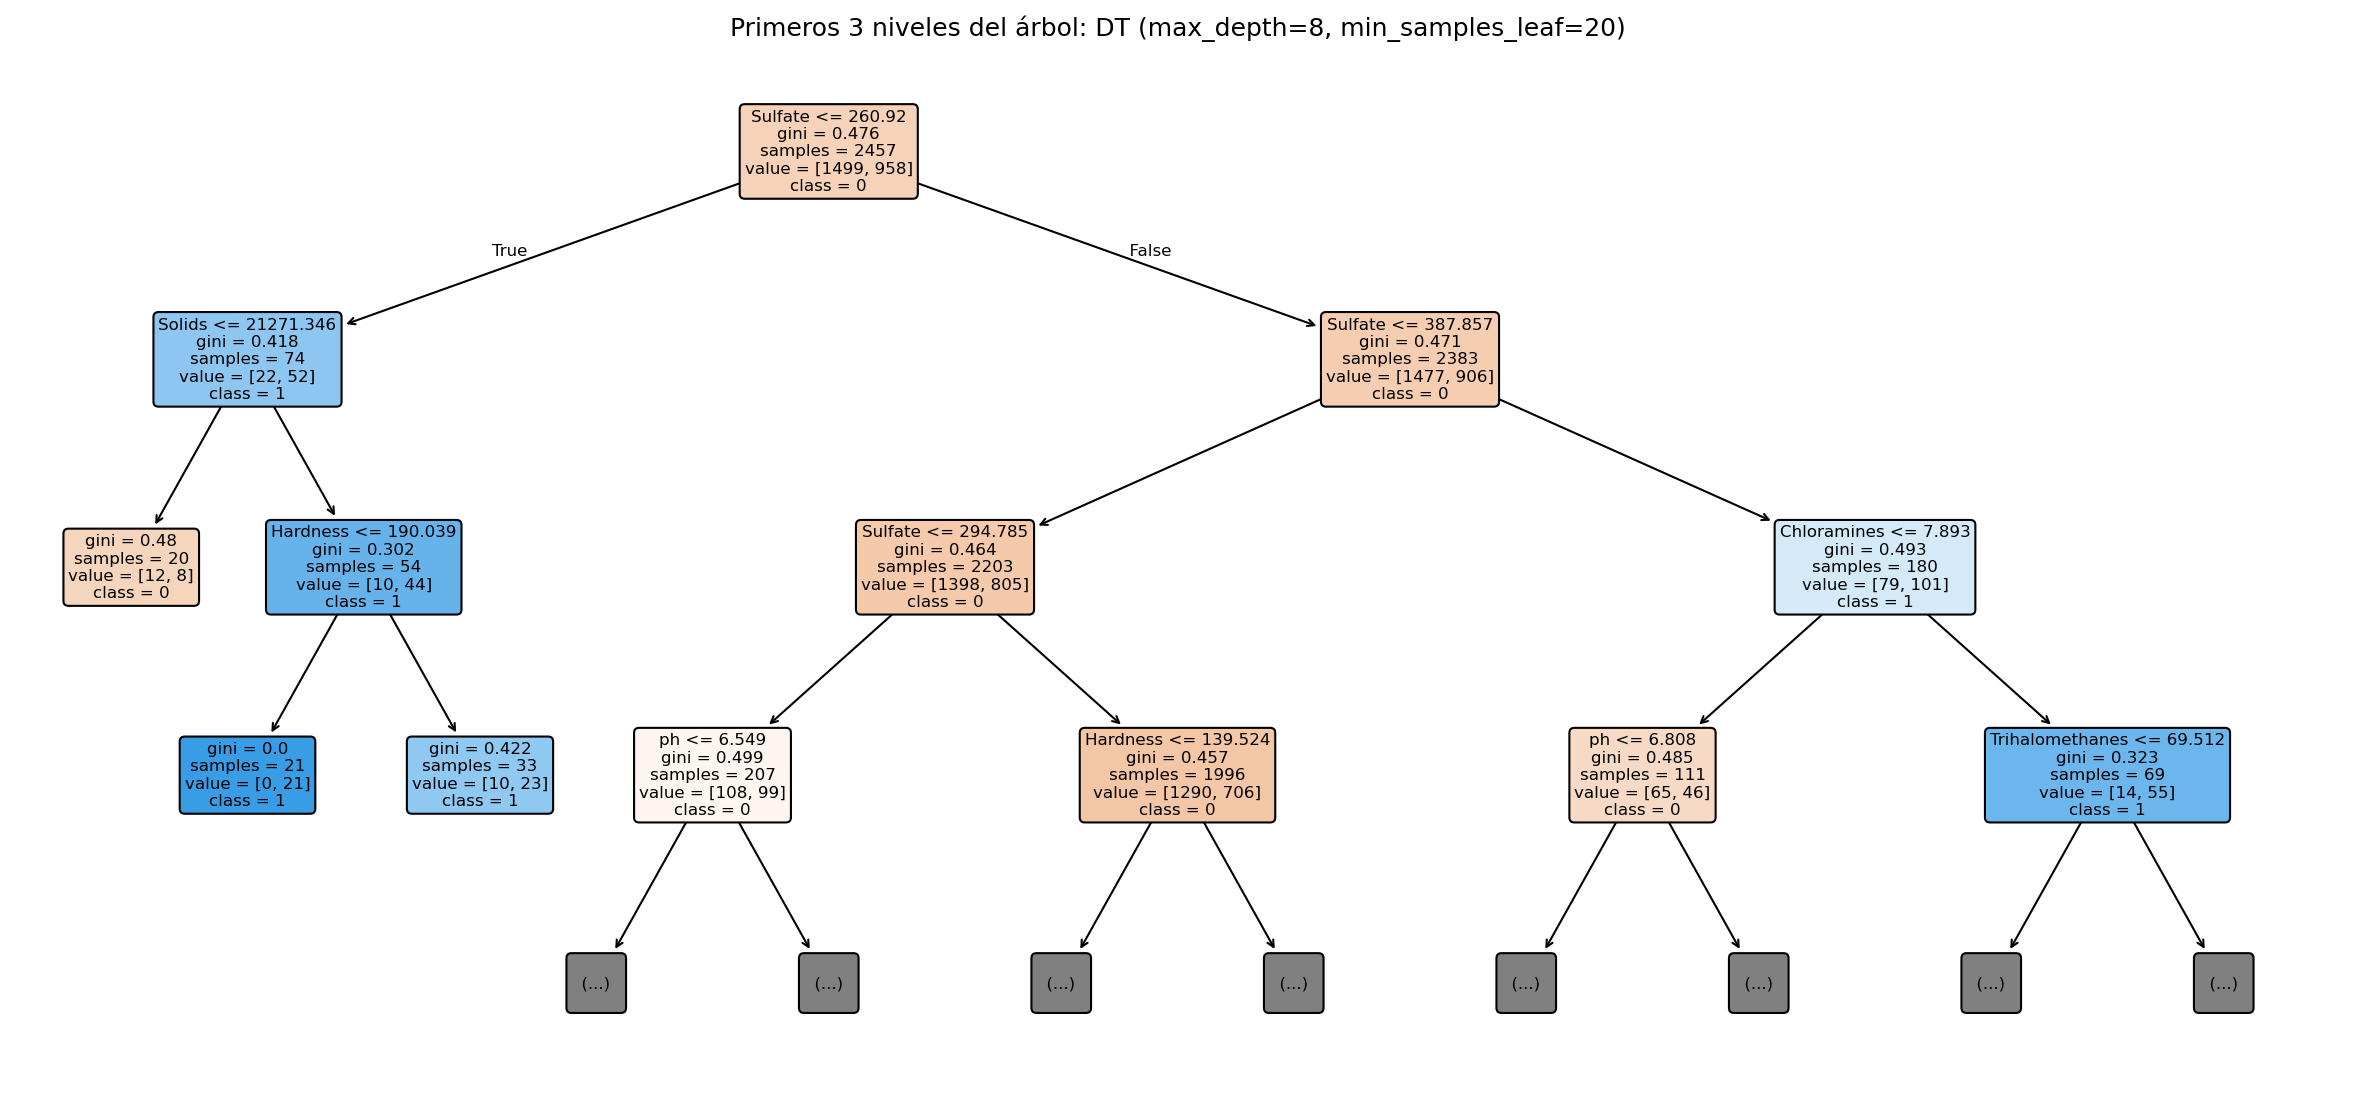
\includegraphics[width=\textwidth]{potabilidad/dt_arbol.png}
\caption{Primeros tres niveles del mejor árbol de decisión.}
\end{figure}

La primera división del árbol es \texttt{Sulfate} $\le 260.9$. Por ahí pasan solo 74 muestras, de las que 52 son potables, y si además \texttt{Solids} $>21\,271$ y \texttt{Hardness} $\le 190$, hay una hoja de 21 muestras todas potables. El árbol encontró zonas pequeñas y extremas donde una clase domina. Eso explica por qué los árboles funcionan algo mejor que KNN aunque no haya correlaciones: las reglas por intervalos captan relaciones no lineales que la correlación no ve \citep{hastie2009}.

\subsection{Random Forest}
La configuración estándar de \citet{breiman2001} en scikit-learn tiene 100 árboles con $\sqrt{p}$ variables por división. Probamos 500 árboles, \textit{bagging} puro (todas las variables en cada división, \citealp{breiman1996}), hojas de al menos 3 individuos, profundidad 12, pesos de clase por muestra bootstrap y selección de 5 atributos.

\begin{table}[H]
\centering
\small
\caption{Configuraciones de Random Forest en potabilidad. La fila en negrita es el mejor modelo según el F1 macro.}
\setlength{\tabcolsep}{4pt}
\begin{tabular}{>{\raggedright\arraybackslash}p{4.9cm}ccccccc}
\toprule
Configuración & PG & Prec.\ 0 & Recall & VPP & F1 & F1 macro & AUC \\
\midrule
estándar & 0.6642 & 0.8818 & 0.3250 & 0.6380 & 0.4306 & 0.5963 & 0.6504 \\
n\_estimators=\allowbreak{}500 & 0.6740 & 0.9038 & 0.3156 & 0.6779 & 0.4307 & 0.6012 & 0.6584 \\
n\_estimators=\allowbreak{}500, \allowbreak max\_features=\allowbreak{}None & 0.6618 & 0.8778 & 0.3250 & 0.6303 & 0.4289 & 0.5943 & 0.6561 \\
n\_estimators=\allowbreak{}500, \allowbreak min\_samples\_leaf=\allowbreak{}3 & 0.6630 & 0.8998 & 0.2938 & 0.6528 & 0.4052 & 0.5850 & 0.6596 \\
n\_estimators=\allowbreak{}500, \allowbreak max\_depth=\allowbreak{}12 & 0.6606 & 0.9339 & 0.2344 & 0.6944 & 0.3505 & 0.5604 & 0.6610 \\
\textbf{n\_estimators=\allowbreak{}500, \allowbreak min\_samples\_leaf=\allowbreak{}5, \allowbreak class\_weight=\allowbreak{}balanced\_subsample} & \textbf{0.6532} & \textbf{0.8236} & \textbf{0.3875} & \textbf{0.5849} & \textbf{0.4662} & \textbf{0.6047} & \textbf{0.6616} \\
5 atributos & 0.6105 & 0.8317 & 0.2656 & 0.5030 & 0.3476 & 0.5350 & 0.5870 \\
\bottomrule
\end{tabular}
\end{table}

Random Forest es el mejor algoritmo en este dataset. Con 500 árboles se obtiene la PG más alta de todo el laboratorio para potabilidad (0.6740). El \textbf{mejor modelo según el F1 macro es el de 500 árboles, \texttt{min\_samples\_leaf}=5 y \texttt{class\_weight}=balanced\_subsample} (F1 macro 0.6047, AUC 0.6616), porque los pesos hacen que detecte más muestras potables (Recall 0.3875) sin perder mucha PG. El \textit{bagging} puro es un poco peor que usar $\sqrt{p}$ variables, lo que confirma que tomar variables al azar ayuda a que los árboles sean distintos entre sí \citep{breiman2001}. Igual que en KNN, quedarse con 5 atributos empeora el modelo (0.5350).

\subsection{XGBoost}
La configuración estándar de \citet{chen2016} tiene 100 árboles, \texttt{learning\_rate}=0.3 y profundidad 6. Las variaciones bajan la tasa de aprendizaje y agregan más árboles, usan submuestreo de filas y columnas, y en la última se agrega \texttt{scale\_pos\_weight}=1.56, que es la relación negativos/positivos del entrenamiento.

\begin{table}[H]
\centering
\small
\caption{Configuraciones de XGBoost en potabilidad. La fila en negrita es el mejor modelo según el F1 macro.}
\setlength{\tabcolsep}{4pt}
\begin{tabular}{>{\raggedright\arraybackslash}p{4.9cm}ccccccc}
\toprule
Configuración & PG & Prec.\ 0 & Recall & VPP & F1 & F1 macro & AUC \\
\midrule
estándar & 0.6252 & 0.7856 & 0.3750 & 0.5286 & 0.4388 & 0.5787 & 0.6194 \\
n\_estimators=\allowbreak{}300, \allowbreak learning\_rate=\allowbreak{}0.05, \allowbreak max\_depth=\allowbreak{}4 & 0.6557 & 0.8677 & 0.3250 & 0.6118 & 0.4245 & 0.5894 & 0.6294 \\
n\_estimators=\allowbreak{}300, \allowbreak learning\_rate=\allowbreak{}0.05, \allowbreak max\_depth=\allowbreak{}6, \allowbreak subsample=\allowbreak{}0.8, \allowbreak colsample\_bytree=\allowbreak{}0.8 & 0.6459 & 0.8357 & 0.3500 & 0.5773 & 0.4358 & 0.5889 & 0.6382 \\
n\_estimators=\allowbreak{}500, \allowbreak learning\_rate=\allowbreak{}0.01, \allowbreak max\_depth=\allowbreak{}6, \allowbreak subsample=\allowbreak{}0.8, \allowbreak colsample\_bytree=\allowbreak{}0.8 & 0.6642 & 0.9058 & 0.2875 & 0.6619 & 0.4009 & 0.5838 & 0.6527 \\
\textbf{n\_estimators=\allowbreak{}300, \allowbreak learning\_rate=\allowbreak{}0.05, \allowbreak max\_depth=\allowbreak{}6, \allowbreak subsample=\allowbreak{}0.8, \allowbreak colsample\_bytree=\allowbreak{}0.8, \allowbreak scale\_pos\_weight=\allowbreak{}1.56} & \textbf{0.6288} & \textbf{0.7435} & \textbf{0.4500} & \textbf{0.5294} & \textbf{0.4865} & \textbf{0.5979} & \textbf{0.6388} \\
\bottomrule
\end{tabular}
\end{table}

Con la configuración estándar, XGBoost sobreajusta (F1 macro 0.5787, AUC 0.6194), algo esperable con una tasa de aprendizaje alta y árboles profundos en datos con tanto ruido \citep{friedman2001}. Bajar la tasa a 0.05 y usar submuestreo mejora la AUC a 0.638. Con 500 árboles y tasa 0.01, la PG sube a 0.6642, pero el modelo se vuelve conservador y su Recall baja a 0.2875. \textbf{El mejor modelo es el que tiene \texttt{scale\_pos\_weight}=1.56}: es el que más muestras potables detecta de todos los mejores modelos (Recall 0.45, 144 de 320) y tiene el segundo mejor F1 macro del dataset (0.5979).

\subsection{AdaBoost}
La configuración estándar de \citet{freund1997} en scikit-learn usa 50 \textit{stumps} con tasa 1. Las variaciones aumentan las iteraciones, bajan la tasa y usan árboles base de profundidad 2, 3 y 4.

\begin{table}[H]
\centering
\small
\caption{Configuraciones de AdaBoost en potabilidad. La fila en negrita es el mejor modelo según el F1 macro.}
\setlength{\tabcolsep}{4pt}
\begin{tabular}{>{\raggedright\arraybackslash}p{4.9cm}ccccccc}
\toprule
Configuración & PG & Prec.\ 0 & Recall & VPP & F1 & F1 macro & AUC \\
\midrule
estándar & 0.6178 & 0.9599 & 0.0844 & 0.5745 & 0.1471 & 0.4504 & 0.5790 \\
n\_estimators=\allowbreak{}200 & 0.6203 & 0.9559 & 0.0969 & 0.5849 & 0.1662 & 0.4602 & 0.5805 \\
n\_estimators=\allowbreak{}200, \allowbreak learning\_rate=\allowbreak{}0.5, \allowbreak profundidad\_base=\allowbreak{}2 & 0.6105 & 0.9198 & 0.1281 & 0.5062 & 0.2045 & 0.4733 & 0.5820 \\
n\_estimators=\allowbreak{}300, \allowbreak learning\_rate=\allowbreak{}0.1, \allowbreak profundidad\_base=\allowbreak{}3 & 0.6288 & 0.9559 & 0.1187 & 0.6333 & 0.2000 & 0.4792 & 0.6158 \\
\textbf{n\_estimators=\allowbreak{}200, \allowbreak learning\_rate=\allowbreak{}0.05, \allowbreak profundidad\_base=\allowbreak{}4} & \textbf{0.6471} & \textbf{0.9639} & \textbf{0.1531} & \textbf{0.7313} & \textbf{0.2532} & \textbf{0.5111} & \textbf{0.6264} \\
\bottomrule
\end{tabular}
\end{table}

AdaBoost es el algoritmo que peor funciona en potabilidad. Con \textit{stumps} solo detecta el 8.4\,\% de las muestras potables, porque cada \textit{stump} hace un solo corte en una variable, y ninguna variable separa las clases por sí sola. Al usar árboles base más profundos (que pueden captar interacciones) y una tasa más baja, el modelo mejora de forma sostenida. \textbf{El mejor es el de 200 iteraciones, tasa 0.05 y profundidad base 4} (F1 macro 0.5111), pero aun así solo detecta el 15.3\,\% de las potables. Este resultado coincide con lo que señalan \citet{hastie2009}: el \textit{boosting} reduce sobre todo el sesgo, pero si el clasificador base no puede representar la estructura de los datos, agregar iteraciones no ayuda.

\subsection{Análisis de los mejores modelos}

\begin{table}[H]
\centering
\small
\caption{Mejor modelo de cada algoritmo en potabilidad, ordenados por F1 macro.}
\setlength{\tabcolsep}{4pt}
\begin{tabular}{>{\raggedright\arraybackslash}p{4.9cm}ccccccc}
\toprule
Modelo & PG & Prec.\ 0 & Recall & VPP & F1 & F1 macro & AUC \\
\midrule
\textbf{RF (n\_estimators=\allowbreak{}500, \allowbreak min\_samples\_leaf=\allowbreak{}5, \allowbreak class\_weight=\allowbreak{}balanced\_subsample)} & \textbf{0.6532} & \textbf{0.8236} & \textbf{0.3875} & \textbf{0.5849} & \textbf{0.4662} & \textbf{0.6047} & \textbf{0.6616} \\
XGBoost (n\_estimators=\allowbreak{}300, \allowbreak learning\_rate=\allowbreak{}0.05, \allowbreak max\_depth=\allowbreak{}6, \allowbreak subsample=\allowbreak{}0.8, \allowbreak colsample\_bytree=\allowbreak{}0.8, \allowbreak scale\_pos\_weight=\allowbreak{}1.56) & 0.6288 & 0.7435 & 0.4500 & 0.5294 & 0.4865 & 0.5979 & 0.6388 \\
DT (max\_depth=\allowbreak{}8, \allowbreak min\_samples\_leaf=\allowbreak{}20) & 0.6557 & 0.8697 & 0.3219 & 0.6131 & 0.4221 & 0.5885 & 0.6304 \\
KNN (estándar) & 0.6093 & 0.7836 & 0.3375 & 0.5000 & 0.4030 & 0.5563 & 0.6037 \\
AdaBoost (n\_estimators=\allowbreak{}200, \allowbreak learning\_rate=\allowbreak{}0.05, \allowbreak profundidad\_base=\allowbreak{}4) & 0.6471 & 0.9639 & 0.1531 & 0.7313 & 0.2532 & 0.5111 & 0.6264 \\
\bottomrule
\end{tabular}
\end{table}

\begin{figure}[H]
\centering
\begin{subfigure}{0.32\textwidth}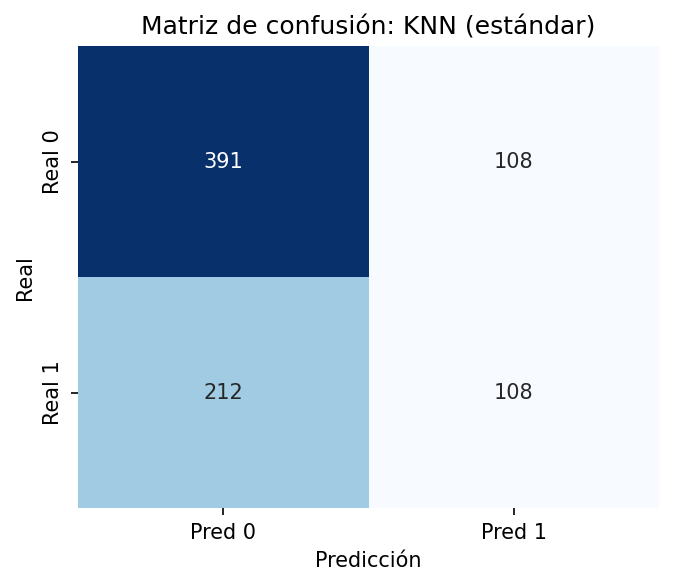
\includegraphics[width=\linewidth]{potabilidad/knn_matriz.png}\caption{KNN}\end{subfigure}
\begin{subfigure}{0.32\textwidth}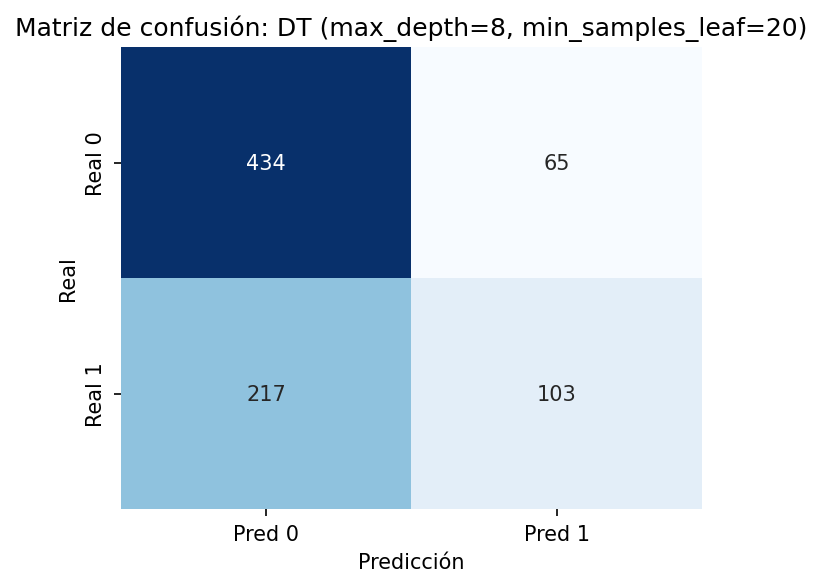
\includegraphics[width=\linewidth]{potabilidad/dt_matriz.png}\caption{DT}\end{subfigure}
\begin{subfigure}{0.32\textwidth}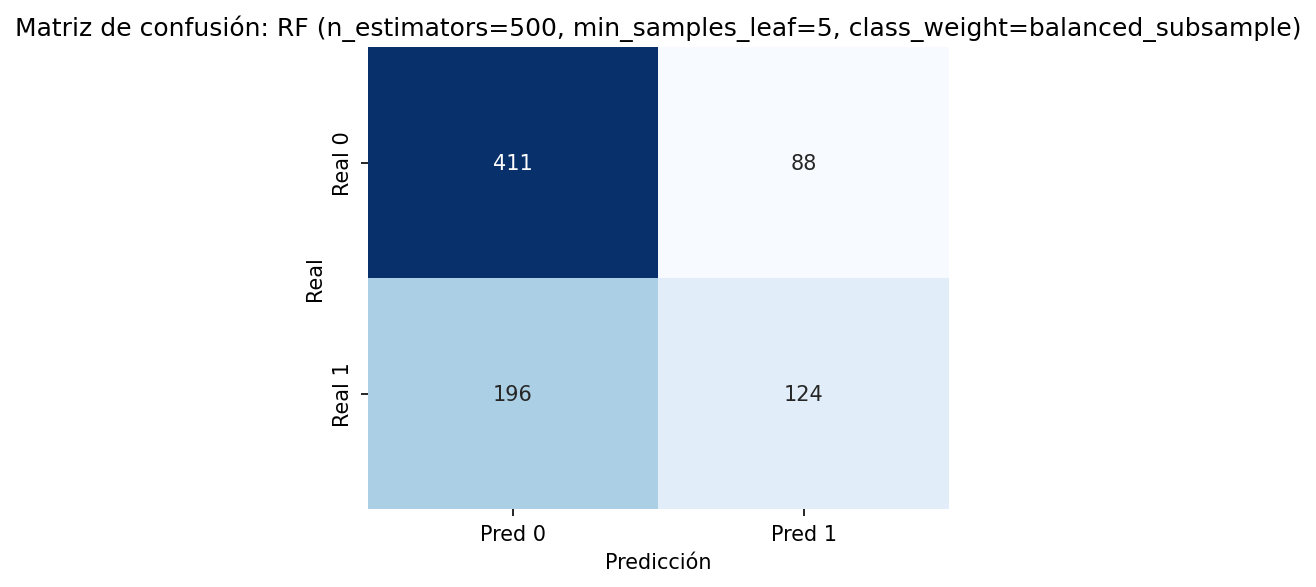
\includegraphics[width=\linewidth]{potabilidad/rf_matriz.png}\caption{RF}\end{subfigure}
\begin{subfigure}{0.32\textwidth}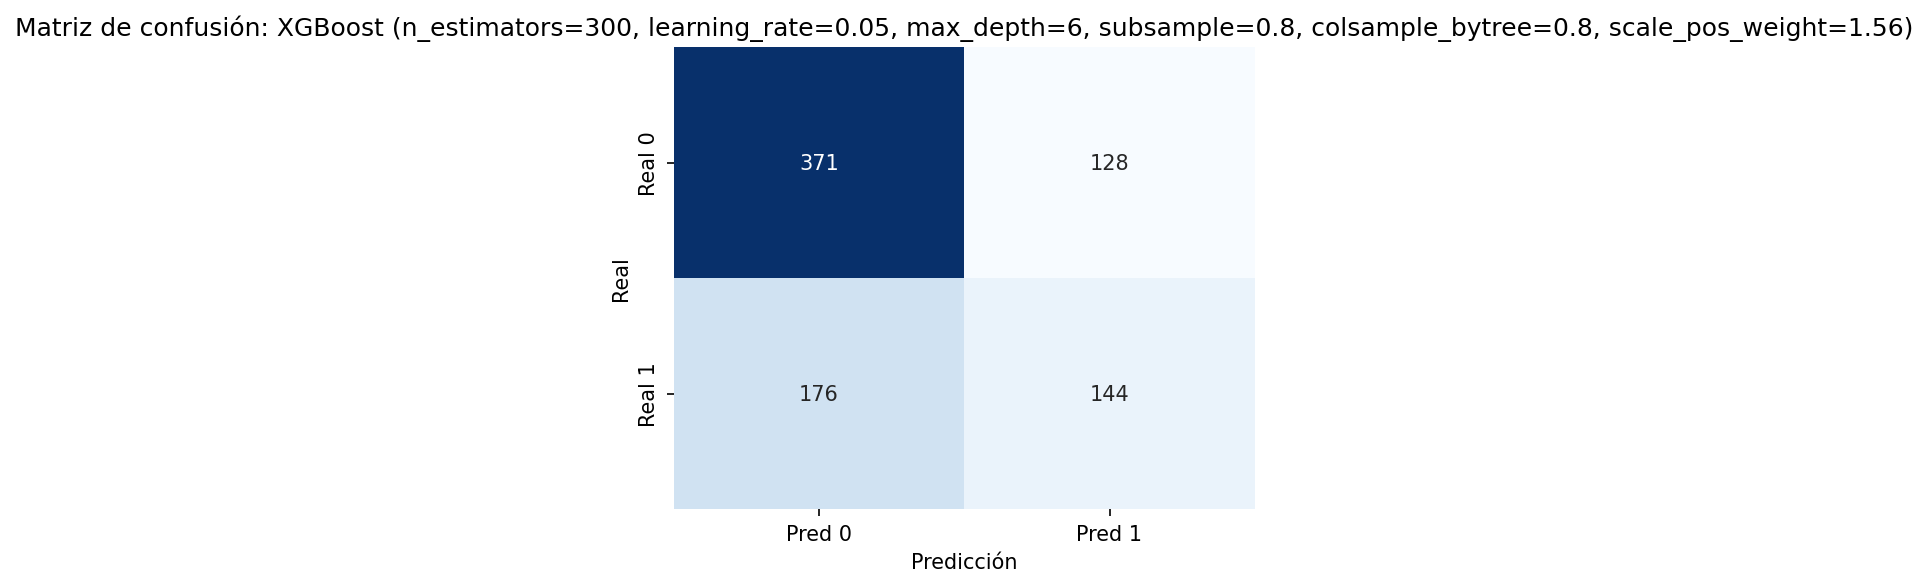
\includegraphics[width=\linewidth]{potabilidad/xgboost_matriz.png}\caption{XGBoost}\end{subfigure}
\begin{subfigure}{0.32\textwidth}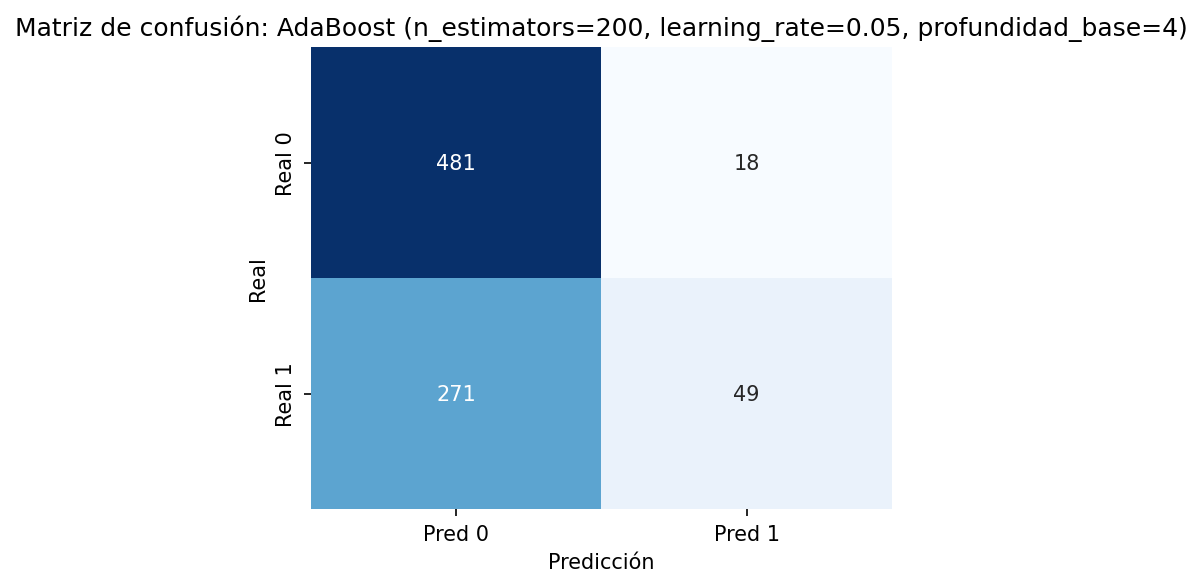
\includegraphics[width=\linewidth]{potabilidad/adaboost_matriz.png}\caption{AdaBoost}\end{subfigure}
\caption{Matrices de confusión del mejor modelo de cada algoritmo (prueba: 499 no potables y 320 potables).}
\end{figure}

Las matrices muestran dos estrategias distintas. AdaBoost casi nunca dice ``potable'': tiene 481 VN y solo 18 FP, pero deja pasar 271 de 320 potables. XGBoost es el que más se arriesga: tiene 144 VP, pero también 128 FP. Random Forest está entre los dos: 124 VP con 88 FP. Lo que conviene depende del costo de cada error, como explican \citet{sokolova2009}. Si un FP significa declarar potable agua que no lo es, el error es grave para la salud, y conviene un modelo con VPP alto como AdaBoost (0.73) o DT (0.61).

\begin{table}[H]
\centering
\caption{Validación cruzada estratificada (5 particiones, sobre el entrenamiento) de los mejores modelos: promedio $\pm$ desviación estándar.}
\begin{tabular}{lcccc}
\toprule
Modelo & PG & F1 & F1 macro & AUC \\
\midrule
\textbf{RF} & \textbf{0.6626 $\pm$ 0.0218} & \textbf{0.4944 $\pm$ 0.0196} & \textbf{0.6205 $\pm$ 0.0189} & \textbf{0.6765 $\pm$ 0.0320} \\
XGBoost & 0.6349 $\pm$ 0.0273 & 0.5058 $\pm$ 0.0400 & 0.6080 $\pm$ 0.0291 & 0.6671 $\pm$ 0.0305 \\
KNN & 0.6345 $\pm$ 0.0148 & 0.4552 $\pm$ 0.0160 & 0.5901 $\pm$ 0.0138 & 0.6319 $\pm$ 0.0278 \\
DT & 0.6349 $\pm$ 0.0128 & 0.3697 $\pm$ 0.0384 & 0.5559 $\pm$ 0.0127 & 0.6181 $\pm$ 0.0253 \\
AdaBoost & 0.6463 $\pm$ 0.0230 & 0.2657 $\pm$ 0.0588 & 0.5163 $\pm$ 0.0360 & 0.6156 $\pm$ 0.0367 \\
\bottomrule
\end{tabular}
\end{table}

La validación cruzada confirma el orden \citep{kohavi1995}: Random Forest sigue siendo el mejor (F1 macro $0.6205\pm0.0189$) y AdaBoost el peor. La única diferencia es que KNN queda por encima del árbol, que en la prueba había quedado mejor. La distancia entre esos dos (0.03) es del mismo tamaño que las desviaciones estándar, así que esa diferencia no es confiable. Todas las AUC están entre 0.61 y 0.68, lo que \citet{fawcett2006} califica como una capacidad de discriminación pobre.

\begin{figure}[H]
\centering
\begin{subfigure}{0.49\textwidth}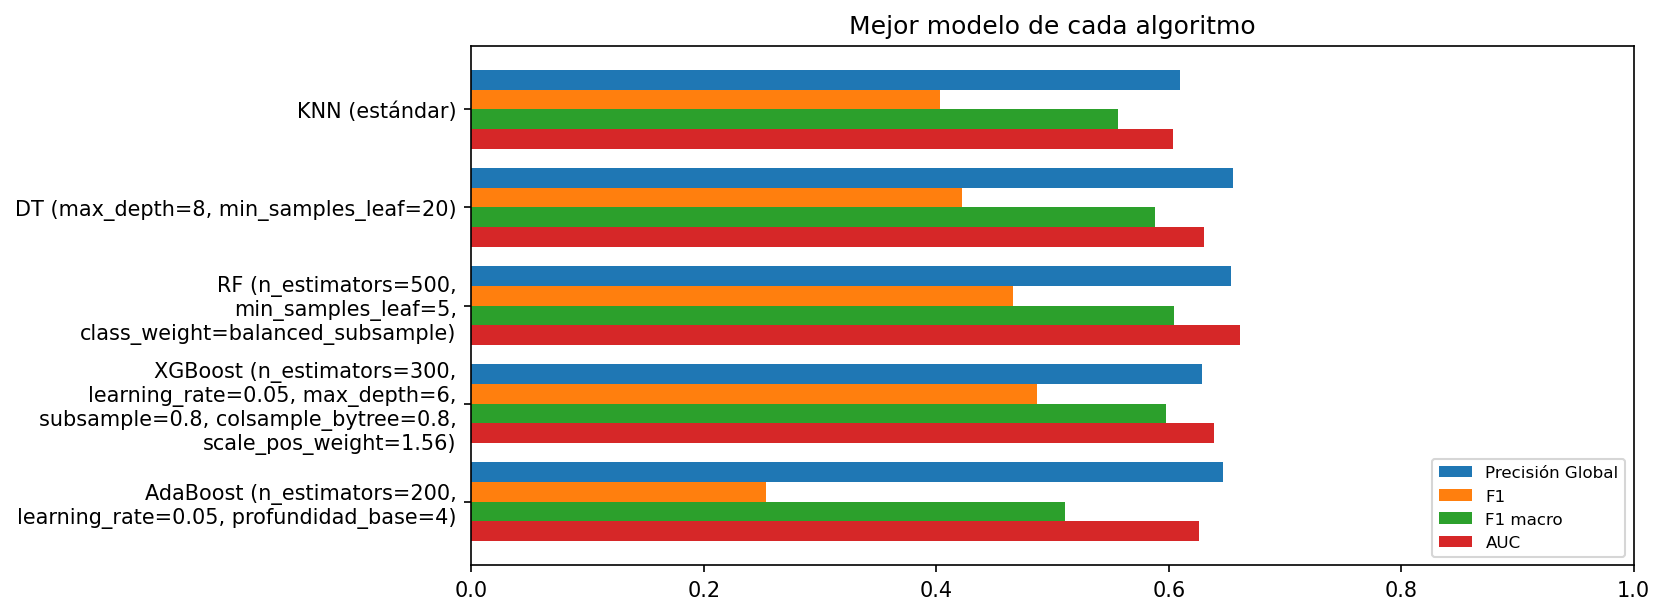
\includegraphics[width=\linewidth]{potabilidad/comparacion_mejores.png}\caption{Índices}\end{subfigure}
\begin{subfigure}{0.43\textwidth}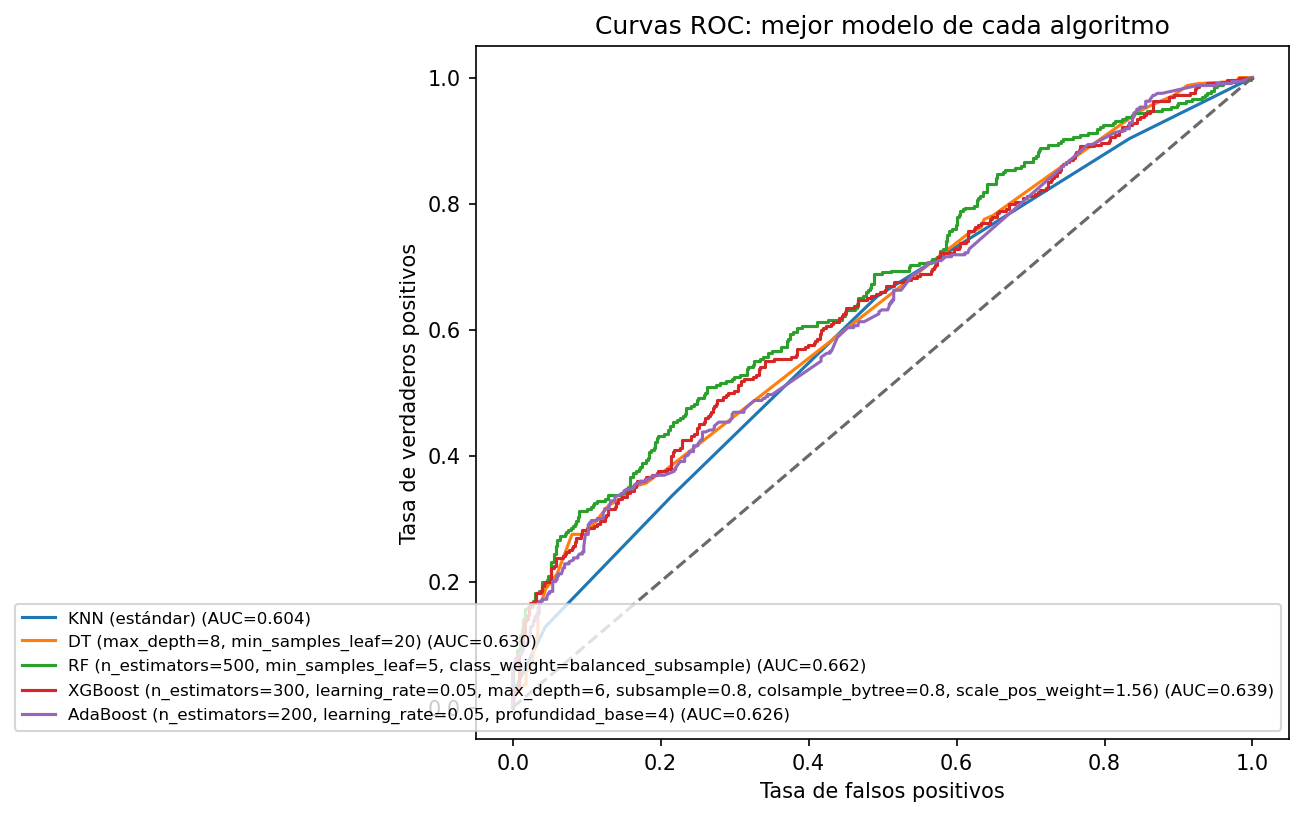
\includegraphics[width=\linewidth]{potabilidad/roc_mejores.png}\caption{Curvas ROC}\end{subfigure}
\caption{Comparación de los mejores modelos de potabilidad.}
\end{figure}

\begin{figure}[H]
\centering
\begin{subfigure}{0.49\textwidth}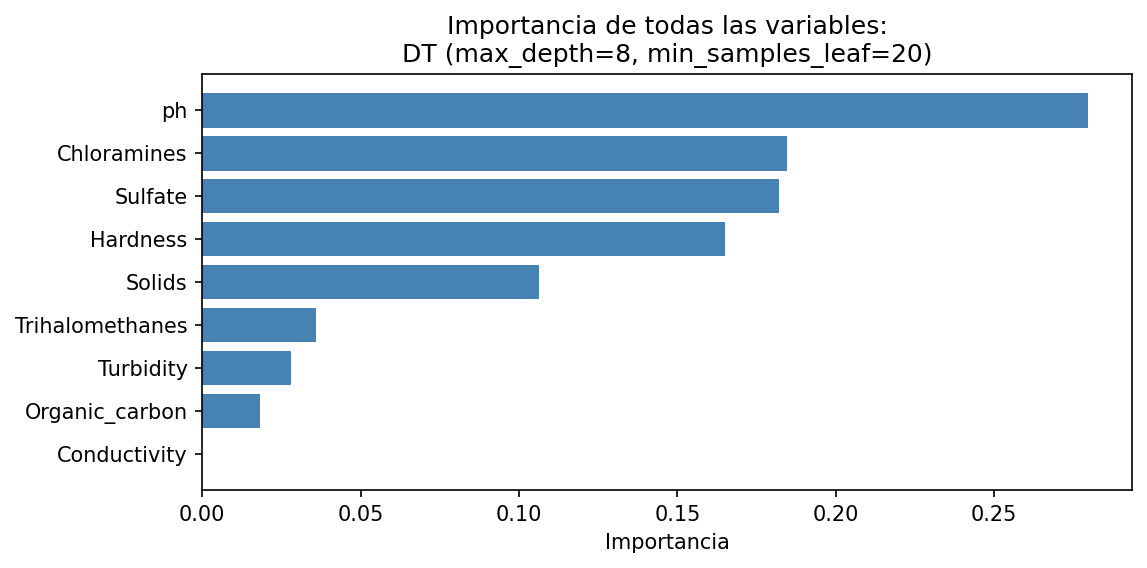
\includegraphics[width=\linewidth]{potabilidad/dt_importancia.png}\caption{DT}\end{subfigure}
\begin{subfigure}{0.49\textwidth}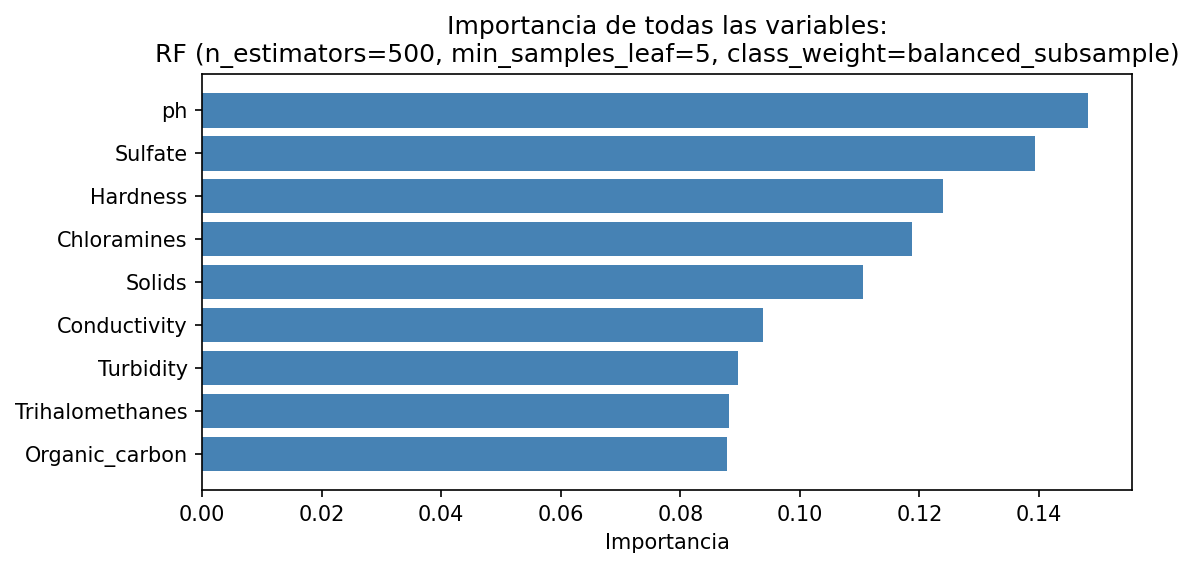
\includegraphics[width=\linewidth]{potabilidad/rf_importancia.png}\caption{RF}\end{subfigure}
\begin{subfigure}{0.49\textwidth}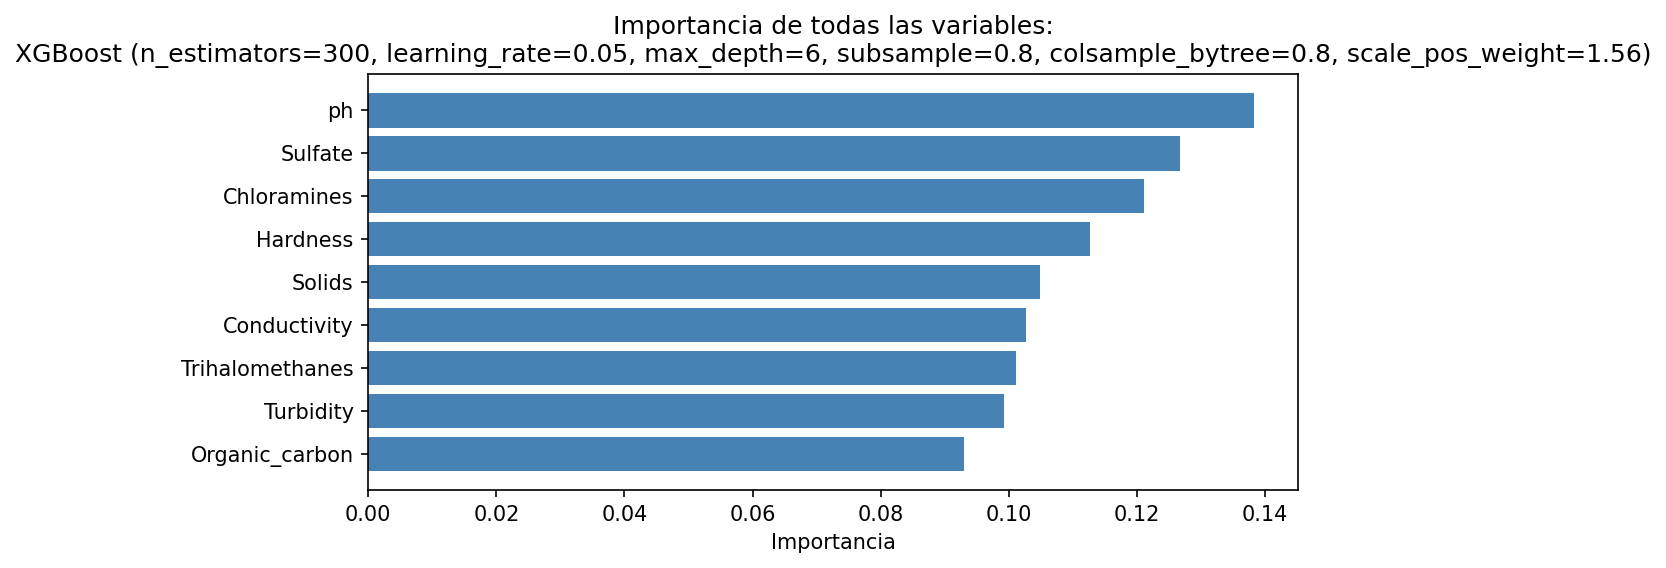
\includegraphics[width=\linewidth]{potabilidad/xgboost_importancia.png}\caption{XGBoost}\end{subfigure}
\begin{subfigure}{0.49\textwidth}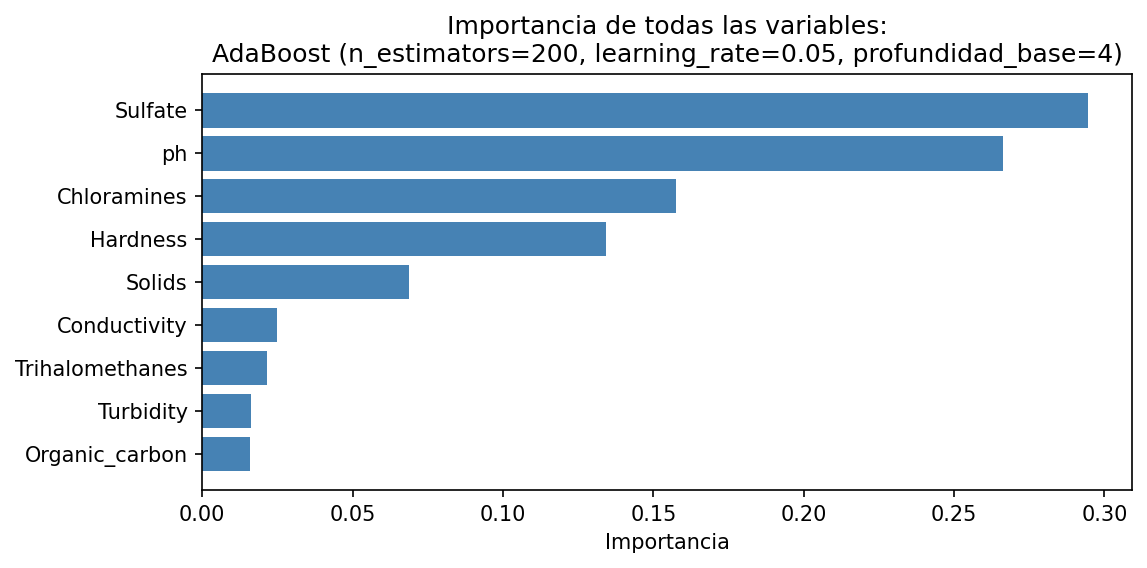
\includegraphics[width=\linewidth]{potabilidad/adaboost_importancia.png}\caption{AdaBoost}\end{subfigure}
\caption{Importancia de las 9 variables en los mejores modelos de árboles.}
\end{figure}

En la importancia de variables, los cuatro modelos de árboles coinciden en que \texttt{ph}, \texttt{Sulfate}, \texttt{Hardness} y \texttt{Chloramines} son las más útiles. Ninguna de esas cuatro estaba entre las más correlacionadas con la clase, lo que confirma que su relación con la potabilidad no es lineal. En Random Forest y XGBoost la importancia está repartida casi por igual (todas entre 0.09 y 0.15), lo que muestra que ninguna variable domina. \textbf{El mejor modelo para potabilidad es Random Forest} con 500 árboles, \texttt{min\_samples\_leaf}=5 y pesos \texttt{balanced\_subsample}, pero su desempeño es apenas moderado.

% ======================================================================
\section{Predicción de diabetes}

\subsection{Análisis exploratorio}
Siguiendo otra vez a \citet{tukey1977}, revisamos primero los datos. No hay valores faltantes, pero sí 3854 filas duplicadas, que se eliminan antes de particionar para que no haya filas iguales en el entrenamiento y en la prueba. Quedan 96\,146 filas: 72\,109 para entrenamiento y 24\,037 para prueba (21\,916 no diabéticos y 2121 diabéticos). El desbalance es fuerte. Solo el 8.5\,\% de los pacientes es diabético, unos 10.34 negativos por cada positivo, y en este tipo de problemas la PG no sirve para comparar modelos \citep{he2009}. \texttt{gender} y \texttt{smoking\_history} se codifican con one-hot dentro del pipeline, lo que da 15 predictoras. La categoría ``No Info'' de \texttt{smoking\_history} es la más frecuente (35\,816 pacientes), y la dejamos como una categoría más en vez de tratarla como faltante.

\begin{figure}[H]
\centering
\begin{subfigure}{0.52\textwidth}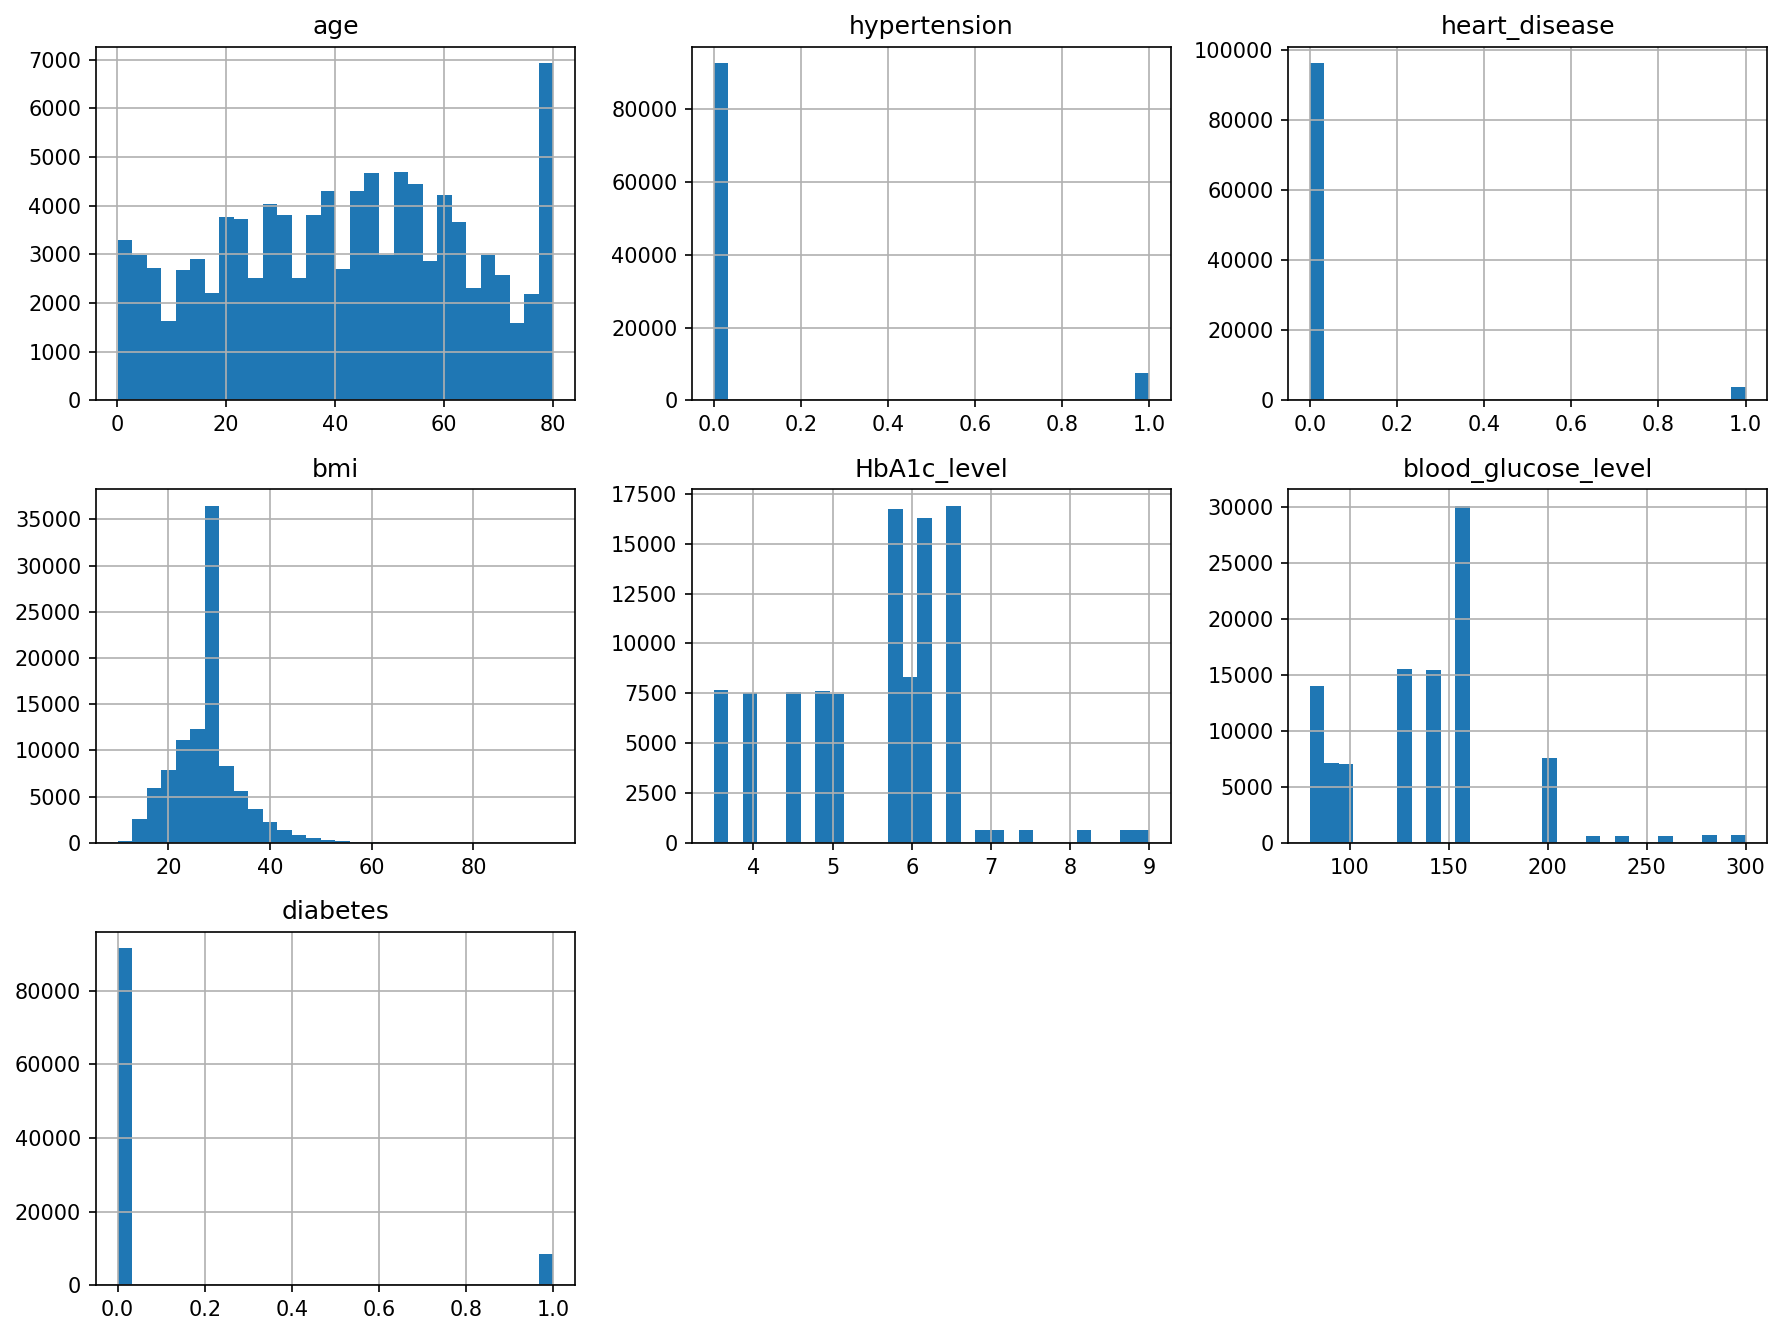
\includegraphics[width=\linewidth]{diabetes/histogramas.png}\caption{Histogramas}\end{subfigure}
\begin{subfigure}{0.46\textwidth}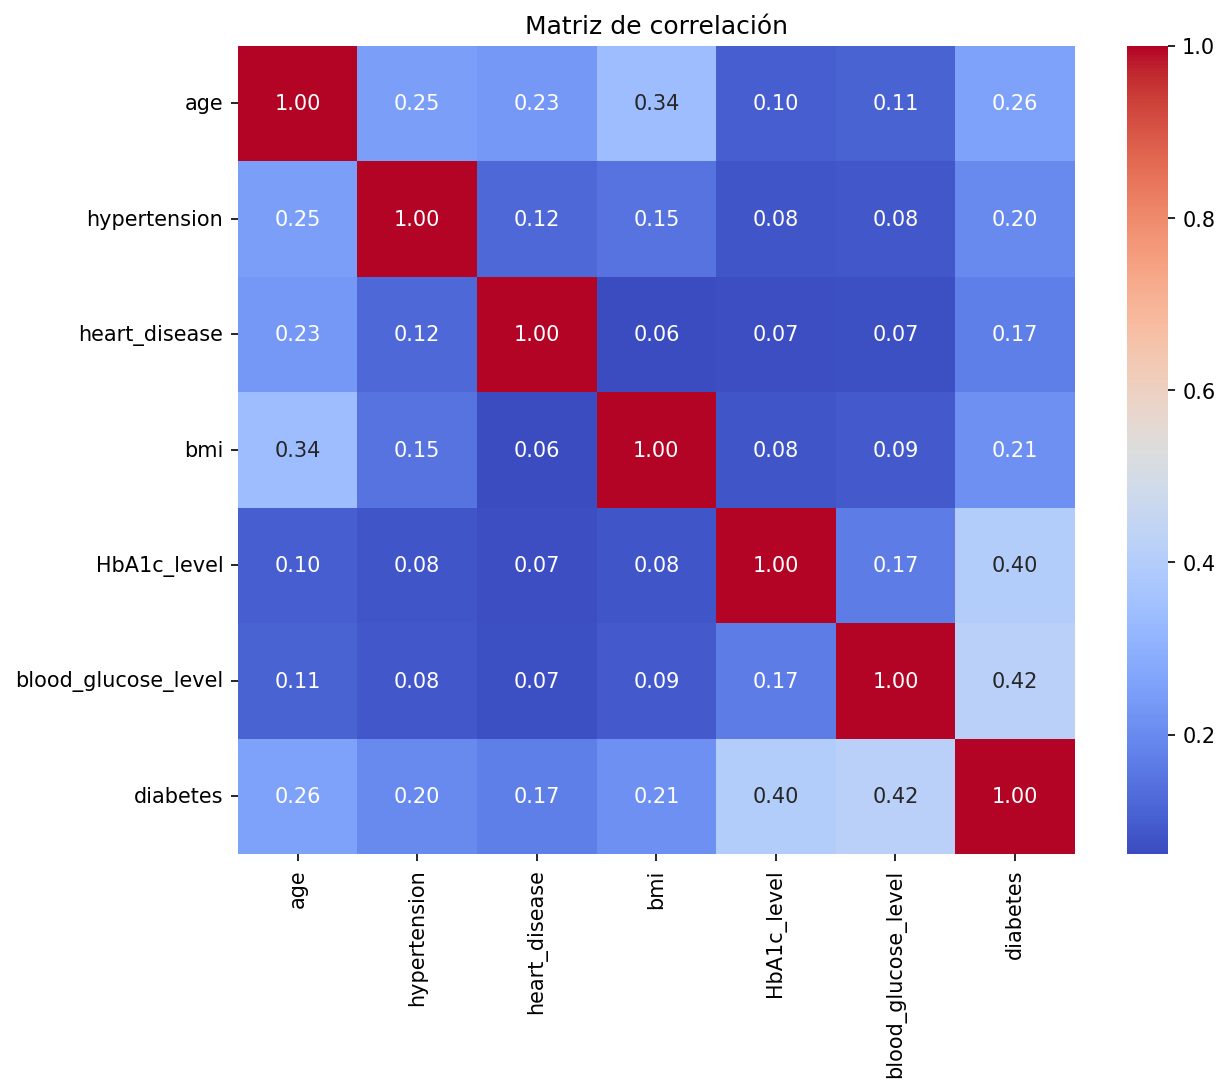
\includegraphics[width=\linewidth]{diabetes/mapa_calor.png}\caption{Mapa de calor}\end{subfigure}
\caption{Distribución y correlaciones de las variables numéricas de diabetes.}
\end{figure}

\begin{figure}[H]
\centering
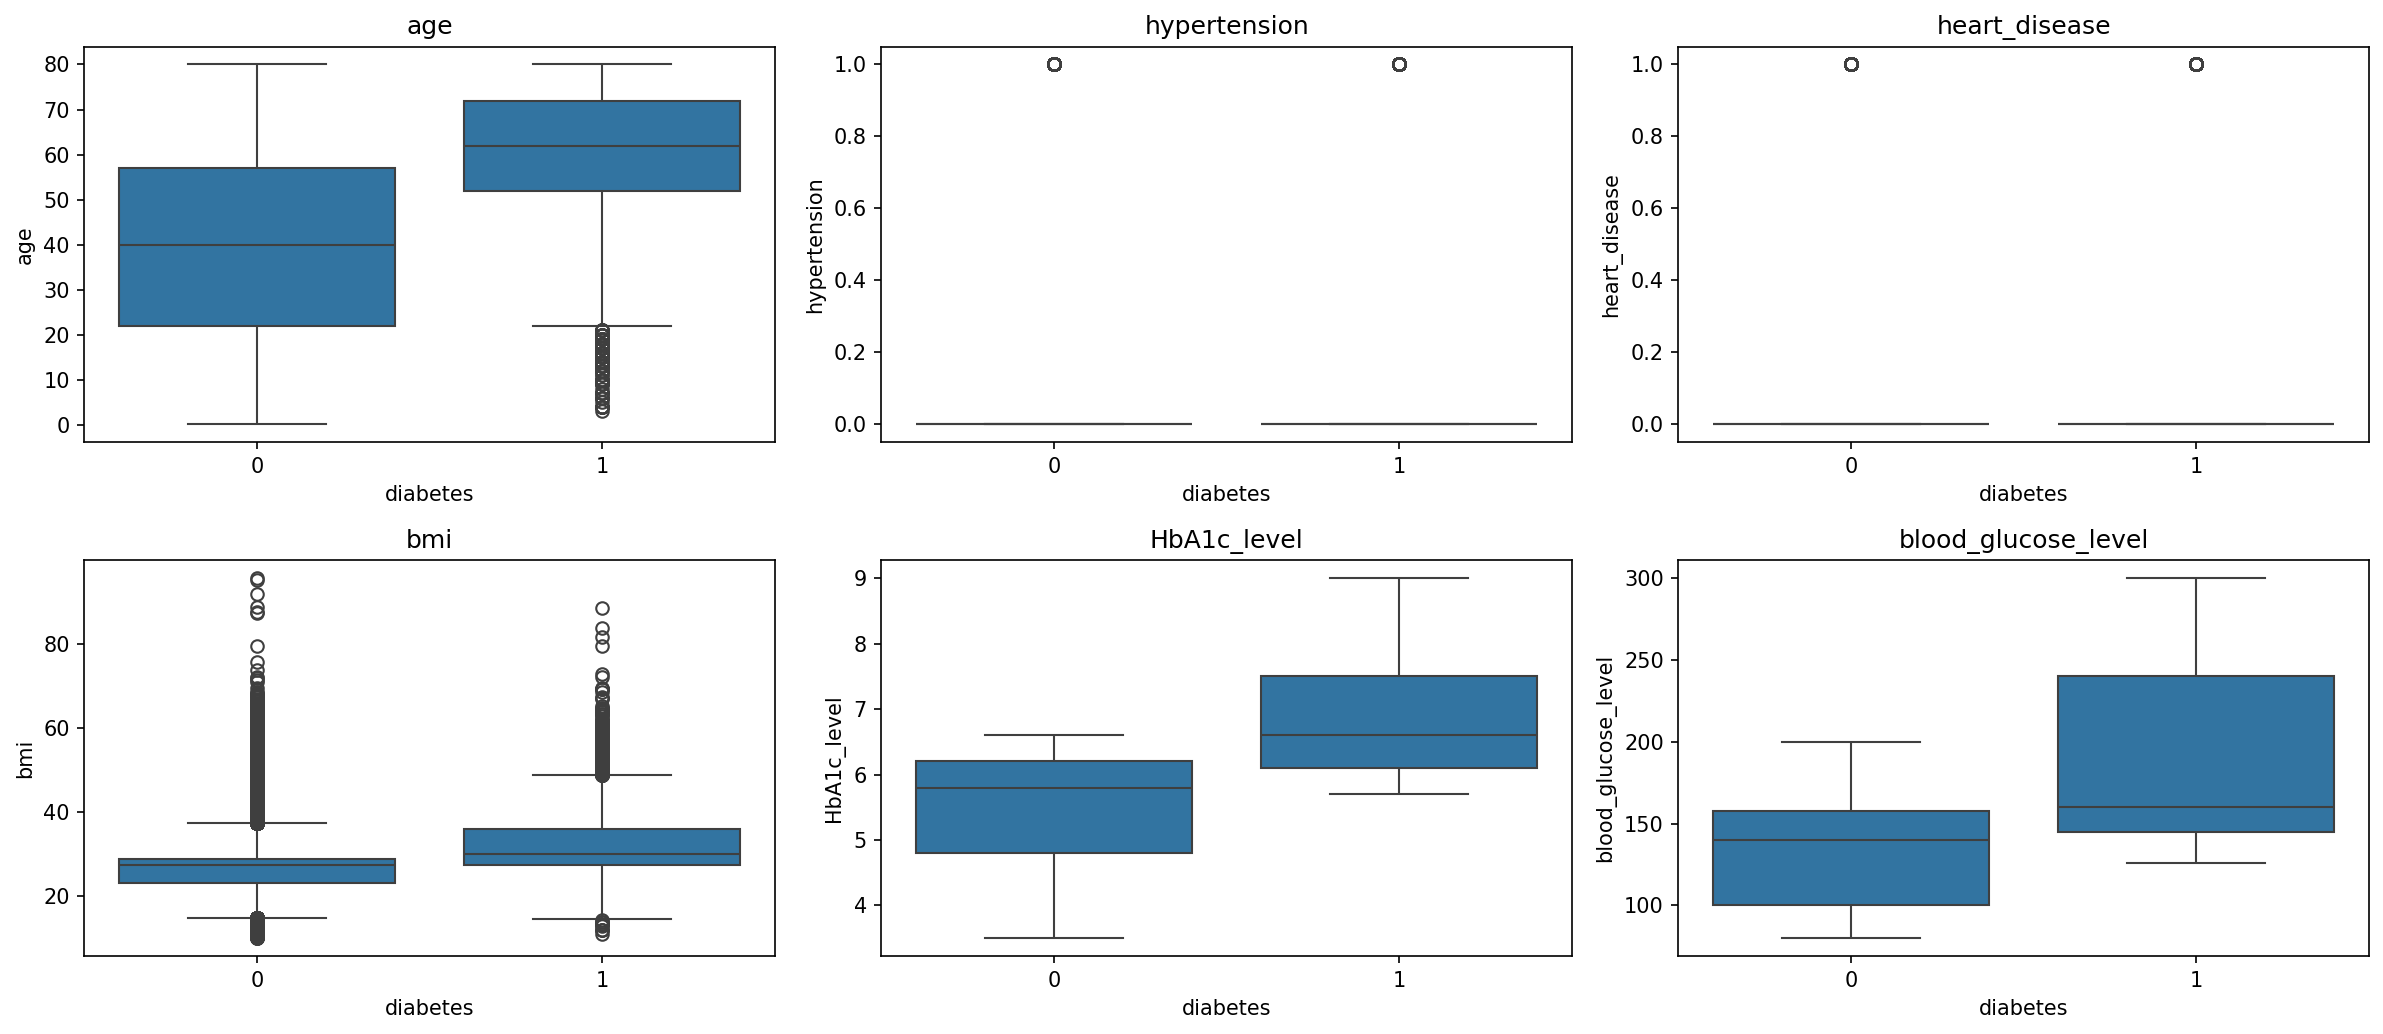
\includegraphics[width=\textwidth]{diabetes/boxplots_clase.png}
\caption{Distribución de cada variable numérica según la clase (0 = no diabético, 1 = diabético).}
\end{figure}

Este dataset es todo lo contrario del anterior. Las variables más correlacionadas con \texttt{diabetes} son \texttt{blood\_glucose\_level} ($r=0.420$) y \texttt{HbA1c\_level} ($r=0.401$), seguidas por \texttt{age} (0.258), \texttt{bmi} (0.214), \texttt{hypertension} (0.198) y \texttt{heart\_disease} (0.172). En el radar, los diabéticos están 1.38 y 1.31 desviaciones estándar por encima de la media en glucosa y HbA1c, y entre 0.56 y 0.85 por encima en las demás variables. En las categóricas, el porcentaje de diabéticos va del 4.1\,\% (``No Info'') al 17.0\,\% (exfumadores, ``former''), y es un poco mayor en hombres (9.75\,\%) que en mujeres (7.62\,\%).

\begin{figure}[H]
\centering
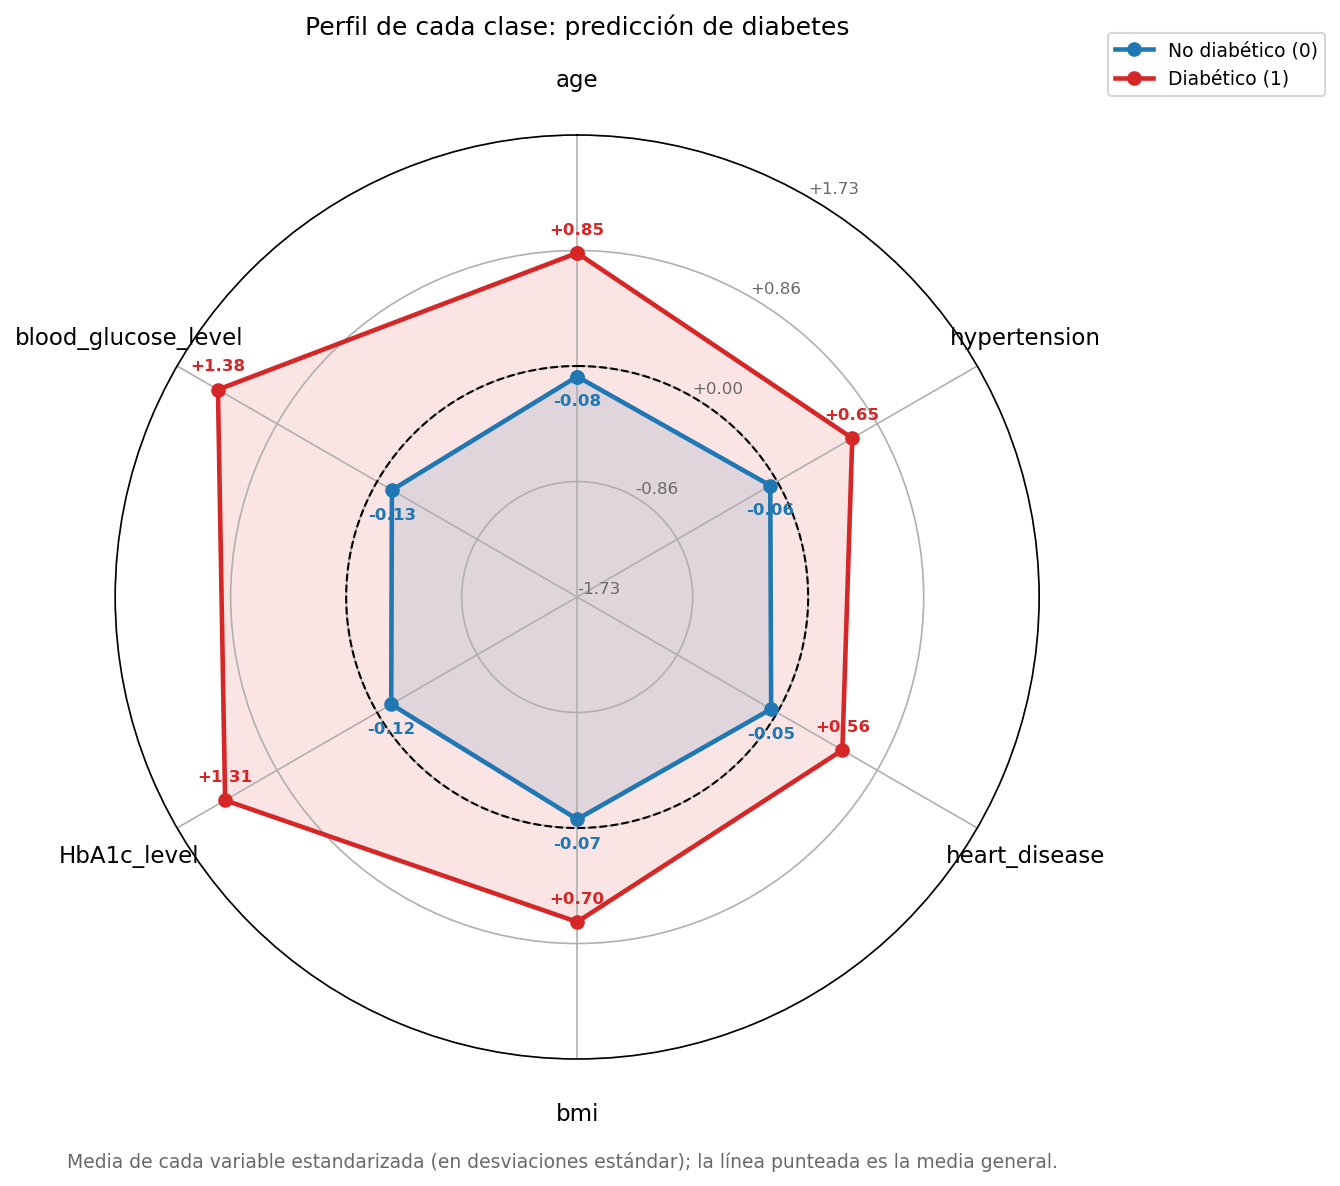
\includegraphics[width=0.68\textwidth]{diabetes/radar_clases.png}
\caption{Radar con la media estandarizada de las 6 variables numéricas en cada clase.}
\end{figure}

Hay un hallazgo que explica casi todos los resultados de esta sección. En los datos sin duplicados, \textbf{ningún paciente no diabético tiene HbA1c mayor que 6.6 ni glucosa mayor que 200}. Los dos valores coinciden con los umbrales de diagnóstico de la \citet{ada2024}: HbA1c $\ge 6.5$\,\% y glucosa al azar $\ge 200$ mg/dL. La regla ``HbA1c $>6.6$ o glucosa $>200$'' identifica al 66.9\,\% de los diabéticos sin ningún falso positivo. El 33\,\% restante tiene valores de HbA1c (5.7 a 6.6) y de glucosa (hasta 200) que también aparecen en los no diabéticos, así que ningún modelo los puede separar bien con estas variables. Como referencia, el clasificador trivial (``nadie es diabético'') tiene una PG de 0.9118 y un F1 macro de 0.477.

\subsection{KNN}
Usamos las mismas configuraciones que en potabilidad \citep{cover1967}, pero con $k=11$ como valor intermedio y selección de 6 atributos. En 72\,000 filas de entrenamiento, $k=11$ todavía es un vecindario muy local.

\begin{table}[H]
\centering
\small
\caption{Configuraciones de KNN en diabetes. La fila en negrita es el mejor modelo según el F1 macro.}
\setlength{\tabcolsep}{4pt}
\begin{tabular}{>{\raggedright\arraybackslash}p{4.9cm}ccccccc}
\toprule
Configuración & PG & Prec.\ 0 & Recall & VPP & F1 & F1 macro & AUC \\
\midrule
estándar & 0.9589 & 0.9925 & 0.6124 & 0.8873 & 0.7247 & 0.8513 & 0.9022 \\
n\_neighbors=\allowbreak{}11 & 0.9599 & 0.9963 & 0.5837 & 0.9393 & 0.7200 & 0.8492 & 0.9325 \\
n\_neighbors=\allowbreak{}25 & 0.9596 & 0.9984 & 0.5587 & 0.9713 & 0.7094 & 0.8438 & 0.9512 \\
n\_neighbors=\allowbreak{}11, \allowbreak weights=\allowbreak{}distance & 0.9599 & 0.9948 & 0.5997 & 0.9171 & 0.7252 & 0.8518 & 0.9306 \\
n\_neighbors=\allowbreak{}11, \allowbreak p=\allowbreak{}1 & 0.9599 & 0.9973 & 0.5743 & 0.9531 & 0.7167 & 0.8476 & 0.9326 \\
n\_neighbors=\allowbreak{}11, \allowbreak sin escalar & 0.9533 & 0.9974 & 0.4974 & 0.9487 & 0.6526 & 0.8138 & 0.9146 \\
\textbf{n\_neighbors=\allowbreak{}11, \allowbreak 6 atributos} & \textbf{0.9647} & \textbf{0.9963} & \textbf{0.6384} & \textbf{0.9436} & \textbf{0.7615} & \textbf{0.8712} & \textbf{0.9343} \\
\bottomrule
\end{tabular}
\end{table}

\begin{figure}[H]
\centering
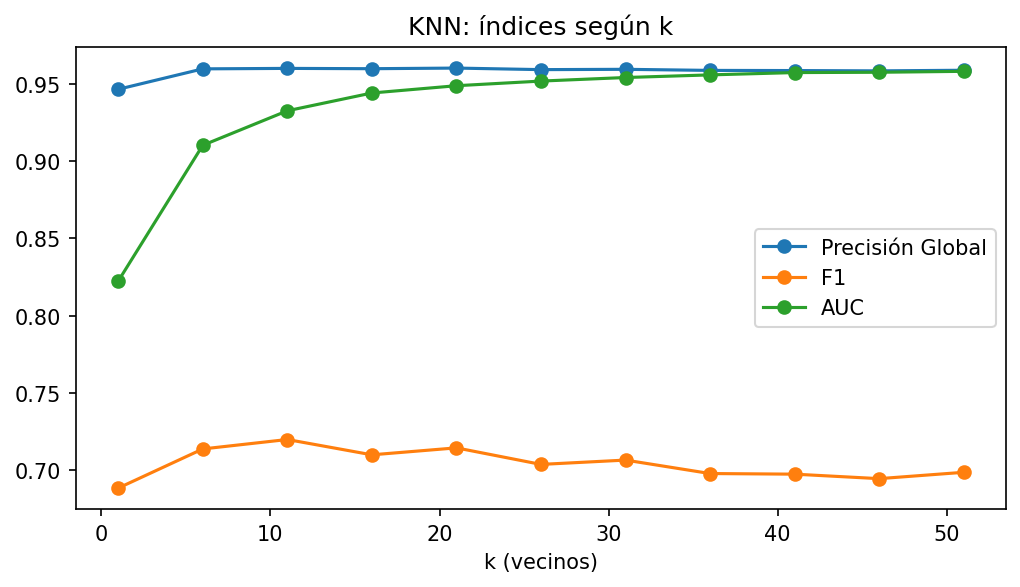
\includegraphics[width=0.7\textwidth]{diabetes/knn_curva_k.png}
\caption{Índices de KNN según la cantidad de vecinos $k$ en diabetes.}
\end{figure}

La curva de $k$ muestra un comportamiento distinto al de potabilidad. La PG casi no cambia (0.946 a 0.960), la AUC sube de forma sostenida (de 0.822 con $k=1$ a 0.958 con $k=51$) y el F1 alcanza su máximo con $k=11$ (0.720). Al usar más vecinos, la probabilidad estimada se vuelve más fina, y por eso la AUC sube, pero con el umbral de 0.5 se detectan menos positivos. En este dataset la selección de atributos sí ayudó, y \textbf{el mejor KNN es $k=11$ con 6 atributos} (F1 macro 0.8712, Recall 0.6384). \texttt{SelectKBest} se quedó con las 6 variables numéricas y quitó las 9 columnas del one-hot. Esas columnas 0/1 agregan dimensiones que no ayudan a separar las clases pero sí cambian las distancias, un problema conocido de los métodos basados en vecinos \citep{guyon2003,hastie2009}. Sin escalar, el F1 macro baja a 0.8138, porque la glucosa, con valores de hasta 300, tapa a la HbA1c.

\subsection{Árboles de Decisión}
Seguimos las mismas ideas de \citet{breiman1984} que en potabilidad, con profundidades 5 y 10 y las mismas opciones de hojas, entropía y pesos de clase.

\begin{table}[H]
\centering
\small
\caption{Configuraciones de Árboles de Decisión en diabetes. La fila en negrita es el mejor modelo según el F1 macro.}
\setlength{\tabcolsep}{4pt}
\begin{tabular}{>{\raggedright\arraybackslash}p{4.9cm}ccccccc}
\toprule
Configuración & PG & Prec.\ 0 & Recall & VPP & F1 & F1 macro & AUC \\
\midrule
estándar & 0.9477 & 0.9682 & 0.7360 & 0.6916 & 0.7131 & 0.8422 & 0.8524 \\
max\_depth=\allowbreak{}5 & 0.9711 & 1.0000 & 0.6728 & 1.0000 & 0.8044 & 0.8944 & 0.9492 \\
max\_depth=\allowbreak{}10 & 0.9709 & 0.9988 & 0.6832 & 0.9817 & 0.8057 & 0.8950 & 0.9712 \\
\textbf{max\_depth=\allowbreak{}10, \allowbreak min\_samples\_leaf=\allowbreak{}20} & \textbf{0.9713} & \textbf{0.9991} & \textbf{0.6836} & \textbf{0.9864} & \textbf{0.8076} & \textbf{0.8960} & \textbf{0.9718} \\
criterion=\allowbreak{}entropy, \allowbreak max\_depth=\allowbreak{}10, \allowbreak min\_samples\_leaf=\allowbreak{}20 & 0.9710 & 0.9992 & 0.6799 & 0.9883 & 0.8056 & 0.8950 & 0.9710 \\
max\_depth=\allowbreak{}10, \allowbreak min\_samples\_leaf=\allowbreak{}20, \allowbreak class\_weight=\allowbreak{}balanced & 0.8828 & 0.8791 & 0.9208 & 0.4243 & 0.5809 & 0.7564 & 0.9721 \\
\bottomrule
\end{tabular}
\end{table}

El árbol estándar creció a 34 niveles y 3313 hojas, y tiene el F1 macro más bajo de los árboles (0.8422), porque genera muchos falsos positivos (VPP 0.6916). Con solo profundidad 5, el árbol ya obtiene una precisión de la clase 0 y un VPP de exactamente 1.0000 con un Recall de 0.6728. O sea, \textbf{aprendió la regla de los umbrales de HbA1c y glucosa}. Con profundidad 10 y hojas de al menos 20 individuos, el árbol quedó con 70 hojas y recuperó unos pocos positivos más de la zona dudosa (Recall 0.6836) a cambio de 20 FP. Es \textbf{el mejor árbol} (F1 macro 0.8960). Con \texttt{class\_weight}=balanced, el Recall sube a 0.92, pero el VPP cae a 0.42.

\begin{figure}[H]
\centering
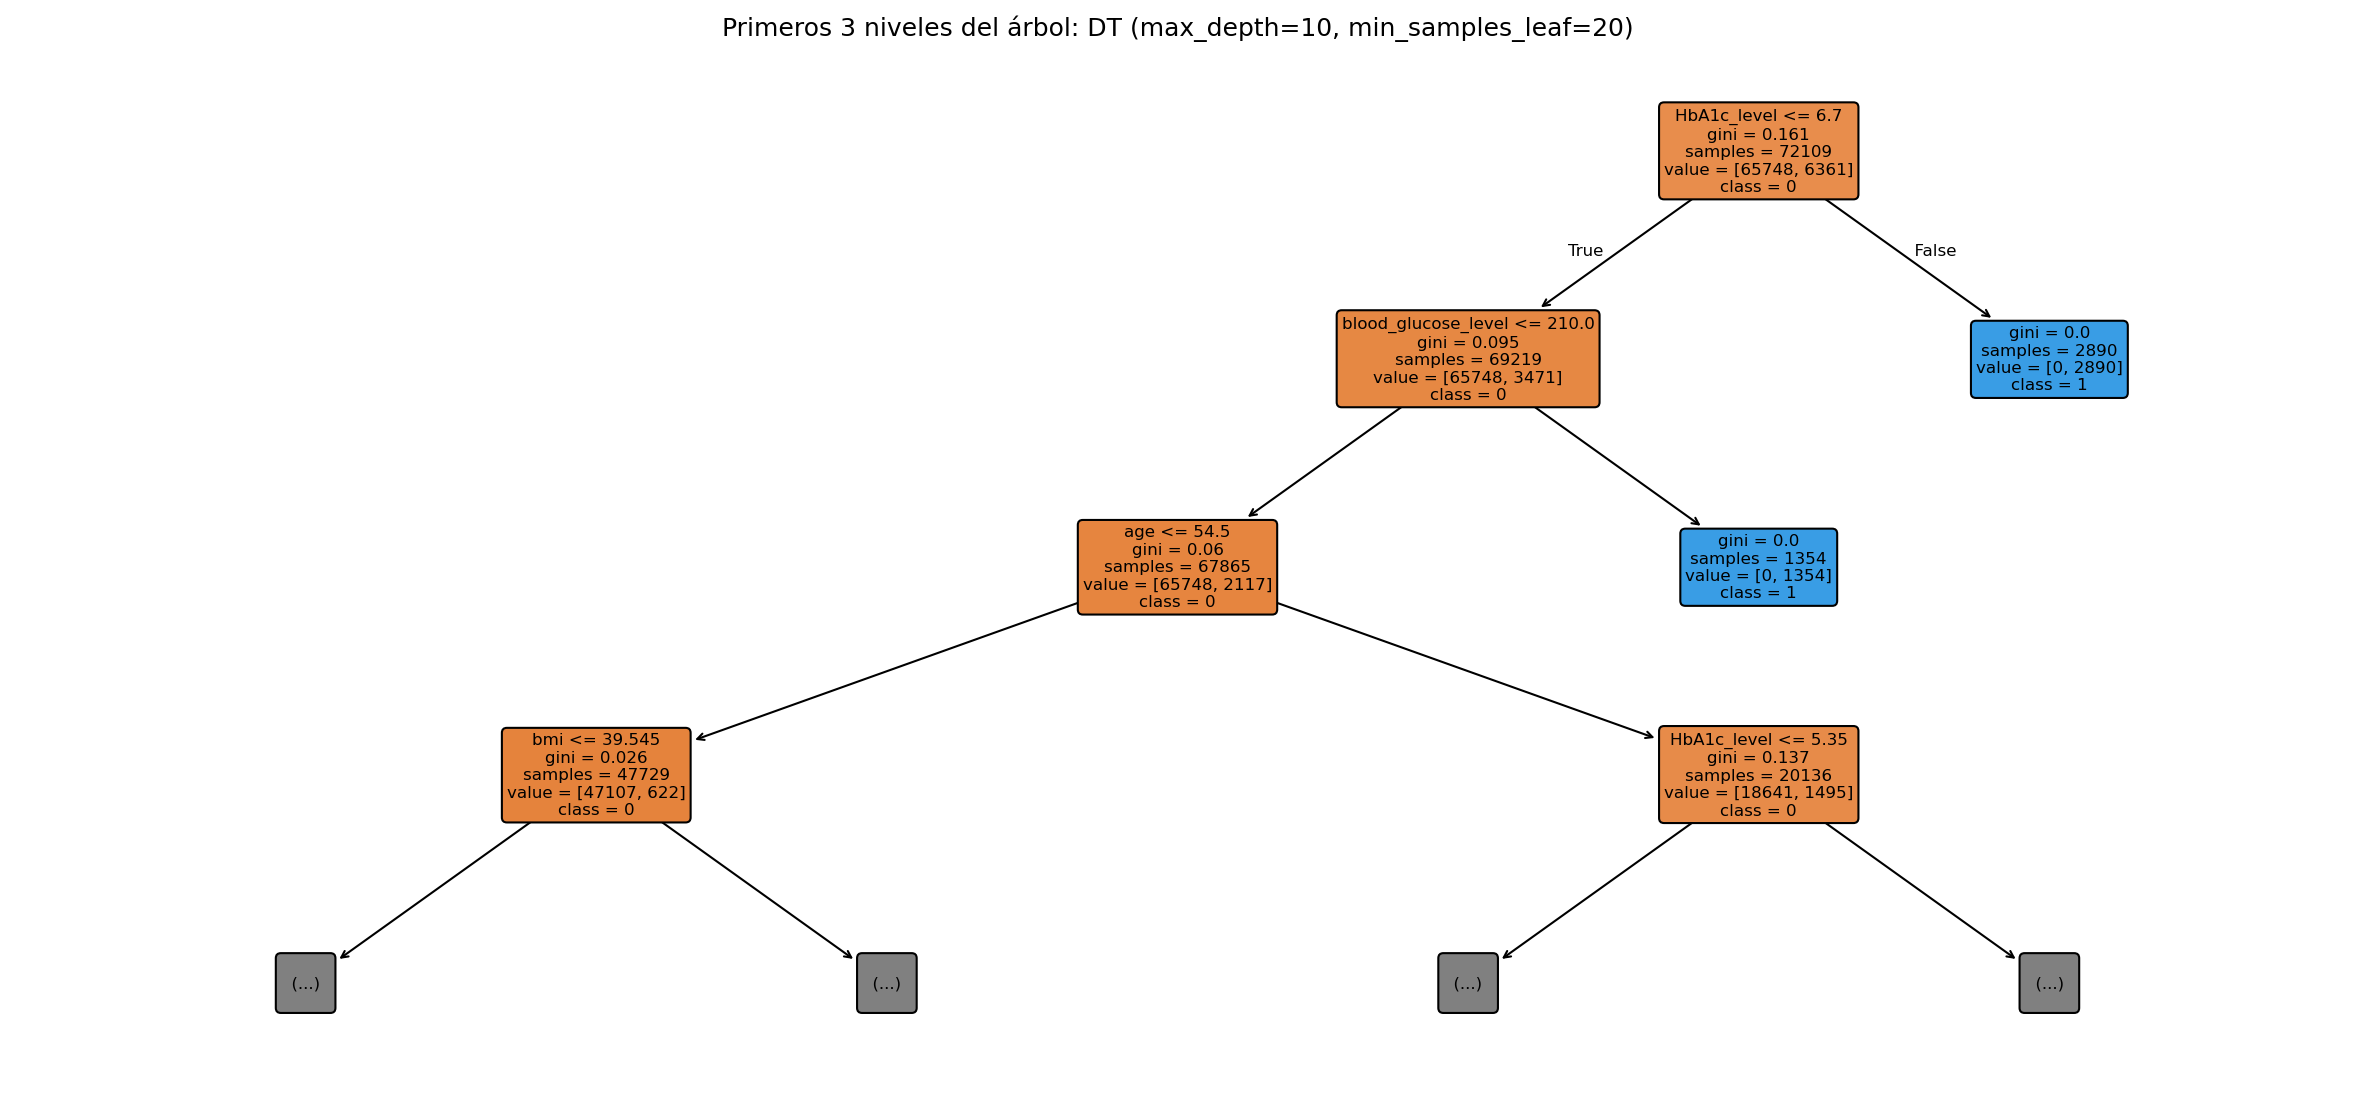
\includegraphics[width=\textwidth]{diabetes/dt_arbol.png}
\caption{Primeros tres niveles del mejor árbol de decisión en diabetes.}
\end{figure}

\subsection{Random Forest}
Usamos las variaciones de \citet{breiman2001} que en potabilidad, pero con 300 árboles, porque este dataset es 30 veces más grande.

\begin{table}[H]
\centering
\small
\caption{Configuraciones de Random Forest en diabetes. La fila en negrita es el mejor modelo según el F1 macro.}
\setlength{\tabcolsep}{4pt}
\begin{tabular}{>{\raggedright\arraybackslash}p{4.9cm}ccccccc}
\toprule
Configuración & PG & Prec.\ 0 & Recall & VPP & F1 & F1 macro & AUC \\
\midrule
estándar & 0.9689 & 0.9963 & 0.6860 & 0.9473 & 0.7957 & 0.8895 & 0.9592 \\
n\_estimators=\allowbreak{}300 & 0.9689 & 0.9963 & 0.6855 & 0.9478 & 0.7956 & 0.8894 & 0.9605 \\
\textbf{n\_estimators=\allowbreak{}300, \allowbreak max\_depth=\allowbreak{}12} & \textbf{0.9713} & \textbf{1.0000} & \textbf{0.6742} & \textbf{1.0000} & \textbf{0.8054} & \textbf{0.8949} & \textbf{0.9704} \\
n\_estimators=\allowbreak{}300, \allowbreak min\_samples\_leaf=\allowbreak{}5 & 0.9712 & 0.9997 & 0.6761 & 0.9958 & 0.8054 & 0.8949 & 0.9693 \\
n\_estimators=\allowbreak{}300, \allowbreak max\_features=\allowbreak{}None & 0.9683 & 0.9942 & 0.7011 & 0.9213 & 0.7963 & 0.8895 & 0.9669 \\
n\_estimators=\allowbreak{}300, \allowbreak max\_depth=\allowbreak{}12, \allowbreak class\_weight=\allowbreak{}balanced\_subsample & 0.9076 & 0.9094 & 0.8897 & 0.4872 & 0.6296 & 0.7884 & 0.9739 \\
6 atributos & 0.9676 & 0.9937 & 0.6973 & 0.9152 & 0.7915 & 0.8870 & 0.9561 \\
\bottomrule
\end{tabular}
\end{table}

El bosque estándar, con árboles sin límite, deja algunos falsos positivos (VPP 0.9473). Al limitar la profundidad a 12, el bosque llega a VPP = 1.0000 y una precisión de la clase 0 de 1.0000, es decir, no tiene ningún falso positivo en 24\,037 pacientes de prueba. Es \textbf{el mejor Random Forest} (F1 macro 0.8949, AUC 0.9704). El \textit{bagging} puro detecta más positivos (Recall 0.7011), pero también tiene más falsos positivos. Seleccionar 6 atributos no mejora el bosque, porque los árboles ya ignoran solos las variables que no sirven \citep{breiman2001}.

\subsection{XGBoost}
Las variaciones de \citet{chen2016} son las mismas que en potabilidad, más dos valores de \texttt{scale\_pos\_weight}: 3 y 10.34 (la relación negativos/positivos).

\begin{table}[H]
\centering
\small
\caption{Configuraciones de XGBoost en diabetes. La fila en negrita es el mejor modelo según el F1 macro.}
\setlength{\tabcolsep}{4pt}
\begin{tabular}{>{\raggedright\arraybackslash}p{4.9cm}ccccccc}
\toprule
Configuración & PG & Prec.\ 0 & Recall & VPP & F1 & F1 macro & AUC \\
\midrule
estándar & 0.9699 & 0.9970 & 0.6898 & 0.9575 & 0.8019 & 0.8928 & 0.9759 \\
\textbf{n\_estimators=\allowbreak{}300, \allowbreak learning\_rate=\allowbreak{}0.05, \allowbreak max\_depth=\allowbreak{}4} & \textbf{0.9714} & \textbf{0.9992} & \textbf{0.6836} & \textbf{0.9884} & \textbf{0.8082} & \textbf{0.8964} & \textbf{0.9779} \\
n\_estimators=\allowbreak{}300, \allowbreak learning\_rate=\allowbreak{}0.05, \allowbreak max\_depth=\allowbreak{}6, \allowbreak subsample=\allowbreak{}0.8, \allowbreak colsample\_bytree=\allowbreak{}0.8 & 0.9706 & 0.9981 & 0.6865 & 0.9726 & 0.8049 & 0.8945 & 0.9775 \\
n\_estimators=\allowbreak{}500, \allowbreak learning\_rate=\allowbreak{}0.1, \allowbreak max\_depth=\allowbreak{}3 & 0.9711 & 0.9983 & 0.6907 & 0.9747 & 0.8085 & 0.8964 & 0.9777 \\
n\_estimators=\allowbreak{}300, \allowbreak learning\_rate=\allowbreak{}0.05, \allowbreak max\_depth=\allowbreak{}4, \allowbreak scale\_pos\_weight=\allowbreak{}3 & 0.9615 & 0.9802 & 0.7690 & 0.7894 & 0.7791 & 0.8790 & 0.9779 \\
n\_estimators=\allowbreak{}300, \allowbreak learning\_rate=\allowbreak{}0.05, \allowbreak max\_depth=\allowbreak{}4, \allowbreak scale\_pos\_weight=\allowbreak{}10.34 & 0.8972 & 0.8948 & 0.9227 & 0.4591 & 0.6131 & 0.7769 & 0.9779 \\
\bottomrule
\end{tabular}
\end{table}

XGBoost tiene las AUC más altas del laboratorio (de 0.9759 a 0.9779). \textbf{El mejor modelo es el de 300 árboles, tasa 0.05 y profundidad 4} (F1 macro 0.8964, el más alto del dataset, y AUC 0.9779). El experimento con \texttt{scale\_pos\_weight} muestra algo importante. Con peso 10.34, el Recall sube de 0.6836 a 0.9227 y el VPP baja de 0.9884 a 0.4591, pero la \textbf{AUC queda exactamente igual} (0.9779). Esto significa que dar más peso a la clase positiva no cambia el orden en que el modelo ordena a los pacientes. Lo que cambia es dónde queda el umbral de decisión \citep{fawcett2006,he2009}. Entonces el peso no hace al modelo mejor ni peor: es una forma de escoger cuántos falsos positivos se aceptan para detectar más diabéticos.

\subsection{AdaBoost}
Las configuraciones de \citet{freund1997} son las mismas que en potabilidad.

\begin{table}[H]
\centering
\small
\caption{Configuraciones de AdaBoost en diabetes. La fila en negrita es el mejor modelo según el F1 macro.}
\setlength{\tabcolsep}{4pt}
\begin{tabular}{>{\raggedright\arraybackslash}p{4.9cm}ccccccc}
\toprule
Configuración & PG & Prec.\ 0 & Recall & VPP & F1 & F1 macro & AUC \\
\midrule
\textbf{estándar} & \textbf{0.9711} & \textbf{1.0000} & \textbf{0.6728} & \textbf{1.0000} & \textbf{0.8044} & \textbf{0.8944} & \textbf{0.9704} \\
n\_estimators=\allowbreak{}200 & 0.9709 & 0.9994 & 0.6766 & 0.9903 & 0.8039 & 0.8941 & 0.9731 \\
n\_estimators=\allowbreak{}200, \allowbreak learning\_rate=\allowbreak{}0.5, \allowbreak profundidad\_base=\allowbreak{}2 & 0.9711 & 0.9999 & 0.6737 & 0.9979 & 0.8044 & 0.8944 & 0.9740 \\
n\_estimators=\allowbreak{}300, \allowbreak learning\_rate=\allowbreak{}0.1, \allowbreak profundidad\_base=\allowbreak{}3 & 0.9711 & 1.0000 & 0.6728 & 1.0000 & 0.8044 & 0.8944 & 0.9743 \\
n\_estimators=\allowbreak{}200, \allowbreak learning\_rate=\allowbreak{}0.05, \allowbreak profundidad\_base=\allowbreak{}4 & 0.9711 & 1.0000 & 0.6728 & 1.0000 & 0.8044 & 0.8944 & 0.9744 \\
\bottomrule
\end{tabular}
\end{table}

Aquí los \textit{stumps} funcionan muy bien. Con dos cortes, uno en HbA1c y otro en glucosa, se reproduce la regla de los umbrales, y por eso la configuración estándar ya tiene VPP = 1.0000 y Recall 0.6728, los mismos índices que el árbol de profundidad 5. Las variaciones dan prácticamente lo mismo (F1 macro entre 0.8941 y 0.8944) y solo mejoran un poco la AUC. Como el F1 macro no cambia, \textbf{se queda como mejor la configuración estándar}, que además es la más simple.

\subsection{Análisis de los mejores modelos}

\begin{table}[H]
\centering
\small
\caption{Mejor modelo de cada algoritmo en diabetes, ordenados por F1 macro.}
\setlength{\tabcolsep}{4pt}
\begin{tabular}{>{\raggedright\arraybackslash}p{4.9cm}ccccccc}
\toprule
Modelo & PG & Prec.\ 0 & Recall & VPP & F1 & F1 macro & AUC \\
\midrule
\textbf{XGBoost (n\_estimators=\allowbreak{}300, \allowbreak learning\_rate=\allowbreak{}0.05, \allowbreak max\_depth=\allowbreak{}4)} & \textbf{0.9714} & \textbf{0.9992} & \textbf{0.6836} & \textbf{0.9884} & \textbf{0.8082} & \textbf{0.8964} & \textbf{0.9779} \\
DT (max\_depth=\allowbreak{}10, \allowbreak min\_samples\_leaf=\allowbreak{}20) & 0.9713 & 0.9991 & 0.6836 & 0.9864 & 0.8076 & 0.8960 & 0.9718 \\
RF (n\_estimators=\allowbreak{}300, \allowbreak max\_depth=\allowbreak{}12) & 0.9713 & 1.0000 & 0.6742 & 1.0000 & 0.8054 & 0.8949 & 0.9704 \\
AdaBoost (estándar) & 0.9711 & 1.0000 & 0.6728 & 1.0000 & 0.8044 & 0.8944 & 0.9704 \\
KNN (n\_neighbors=\allowbreak{}11, \allowbreak 6 atributos) & 0.9647 & 0.9963 & 0.6384 & 0.9436 & 0.7615 & 0.8712 & 0.9343 \\
\bottomrule
\end{tabular}
\end{table}

\begin{figure}[H]
\centering
\begin{subfigure}{0.32\textwidth}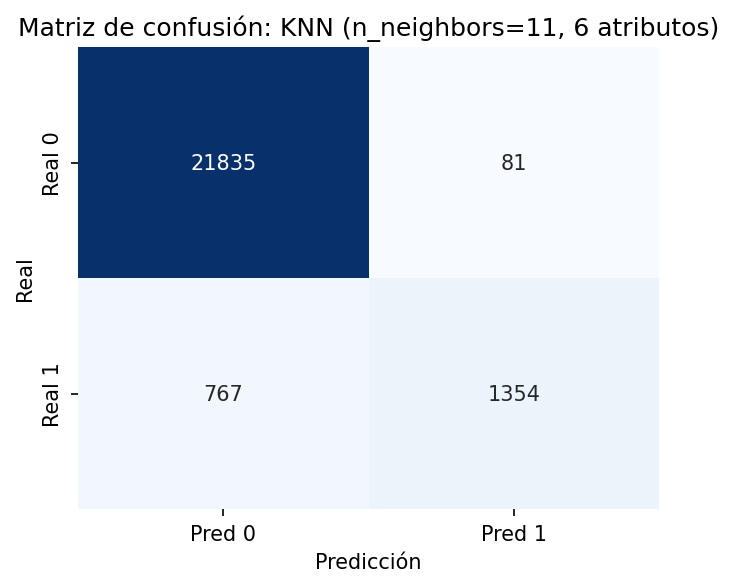
\includegraphics[width=\linewidth]{diabetes/knn_matriz.png}\caption{KNN}\end{subfigure}
\begin{subfigure}{0.32\textwidth}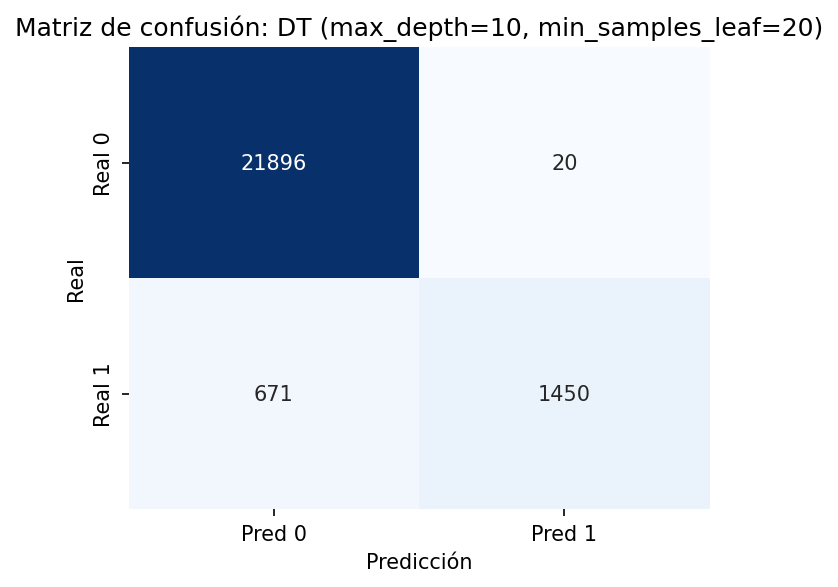
\includegraphics[width=\linewidth]{diabetes/dt_matriz.png}\caption{DT}\end{subfigure}
\begin{subfigure}{0.32\textwidth}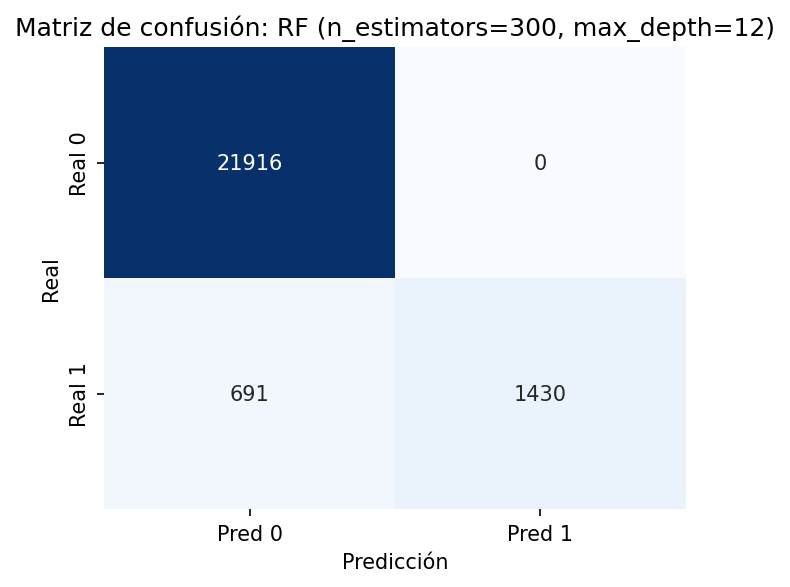
\includegraphics[width=\linewidth]{diabetes/rf_matriz.png}\caption{RF}\end{subfigure}
\begin{subfigure}{0.32\textwidth}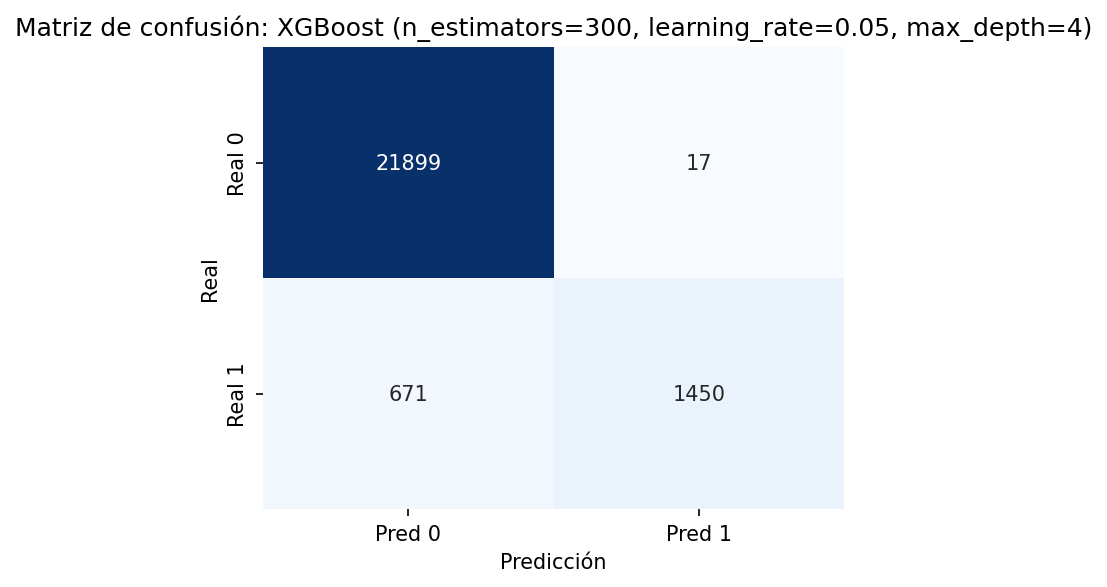
\includegraphics[width=\linewidth]{diabetes/xgboost_matriz.png}\caption{XGBoost}\end{subfigure}
\begin{subfigure}{0.32\textwidth}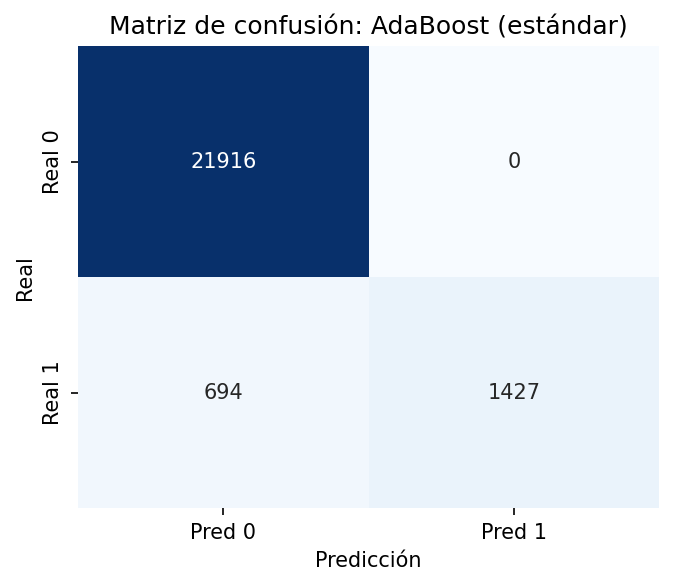
\includegraphics[width=\linewidth]{diabetes/adaboost_matriz.png}\caption{AdaBoost}\end{subfigure}
\caption{Matrices de confusión del mejor modelo de cada algoritmo (prueba: 21\,916 no diabéticos y 2121 diabéticos).}
\end{figure}

Las matrices de los cuatro modelos de árboles son casi iguales. Random Forest y AdaBoost no tienen ningún falso positivo y detectan 1430 y 1427 de los 2121 diabéticos. XGBoost y DT detectan 1450 con solo 17 y 20 FP. Todos dejan sin detectar unos 670 a 690 diabéticos, que son justamente los que están en la zona donde las clases se traslapan. KNN es el único claramente peor (767 FN y 81 FP), lo que concuerda con lo que dicen \citet{hastie2009} sobre los métodos de vecinos cuando hay variables binarias y de escalas distintas.

\begin{table}[H]
\centering
\caption{Validación cruzada estratificada (5 particiones, sobre el entrenamiento) de los mejores modelos en diabetes: promedio $\pm$ desviación estándar.}
\begin{tabular}{lcccc}
\toprule
Modelo & PG & F1 & F1 macro & AUC \\
\midrule
\textbf{XGBoost} & \textbf{0.9708 $\pm$ 0.0008} & \textbf{0.8043 $\pm$ 0.0064} & \textbf{0.8943 $\pm$ 0.0034} & \textbf{0.9794 $\pm$ 0.0016} \\
DT & 0.9703 $\pm$ 0.0008 & 0.8015 $\pm$ 0.0066 & 0.8927 $\pm$ 0.0035 & 0.9742 $\pm$ 0.0023 \\
RF & 0.9706 $\pm$ 0.0008 & 0.8005 $\pm$ 0.0065 & 0.8923 $\pm$ 0.0035 & 0.9724 $\pm$ 0.0026 \\
AdaBoost & 0.9706 $\pm$ 0.0008 & 0.8004 $\pm$ 0.0061 & 0.8923 $\pm$ 0.0032 & 0.9726 $\pm$ 0.0028 \\
KNN & 0.9648 $\pm$ 0.0003 & 0.7603 $\pm$ 0.0038 & 0.8706 $\pm$ 0.0020 & 0.9402 $\pm$ 0.0038 \\
\bottomrule
\end{tabular}
\end{table}

La validación cruzada da el mismo orden que el conjunto de prueba, con desviaciones estándar muy pequeñas (menos de 0.004 en el F1 macro), así que los resultados son estables \citep{kohavi1995}. Sin embargo, entre XGBoost, DT, RF y AdaBoost las diferencias de F1 macro (de 0.0016 a 0.0020) son menores que una desviación estándar, así que en la práctica los cuatro empatan. Donde XGBoost sí se separa es en la AUC ($0.9794\pm0.0016$ contra 0.974 del siguiente), o sea, ordena mejor a los pacientes por riesgo. Según \citet{fawcett2006}, todas las AUC por encima de 0.97 indican una discriminación excelente.

\begin{figure}[H]
\centering
\begin{subfigure}{0.49\textwidth}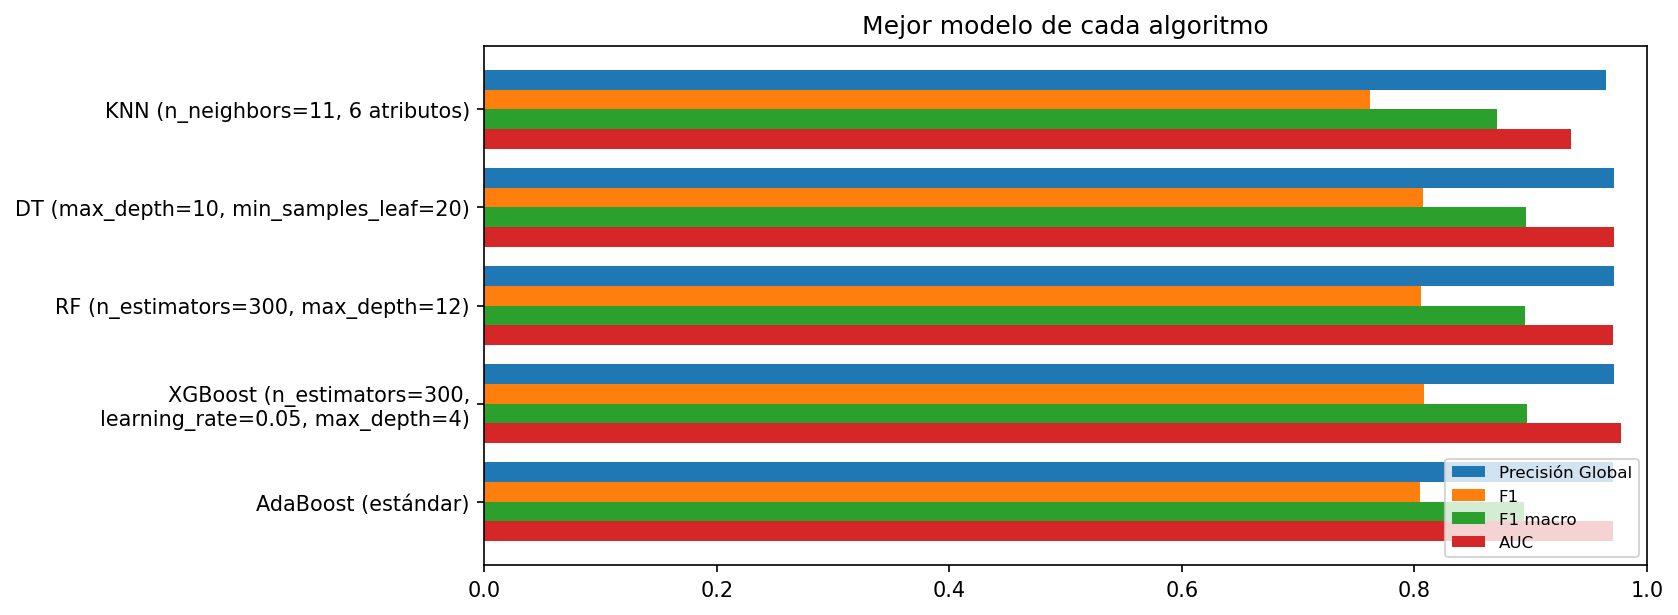
\includegraphics[width=\linewidth]{diabetes/comparacion_mejores.png}\caption{Índices}\end{subfigure}
\begin{subfigure}{0.43\textwidth}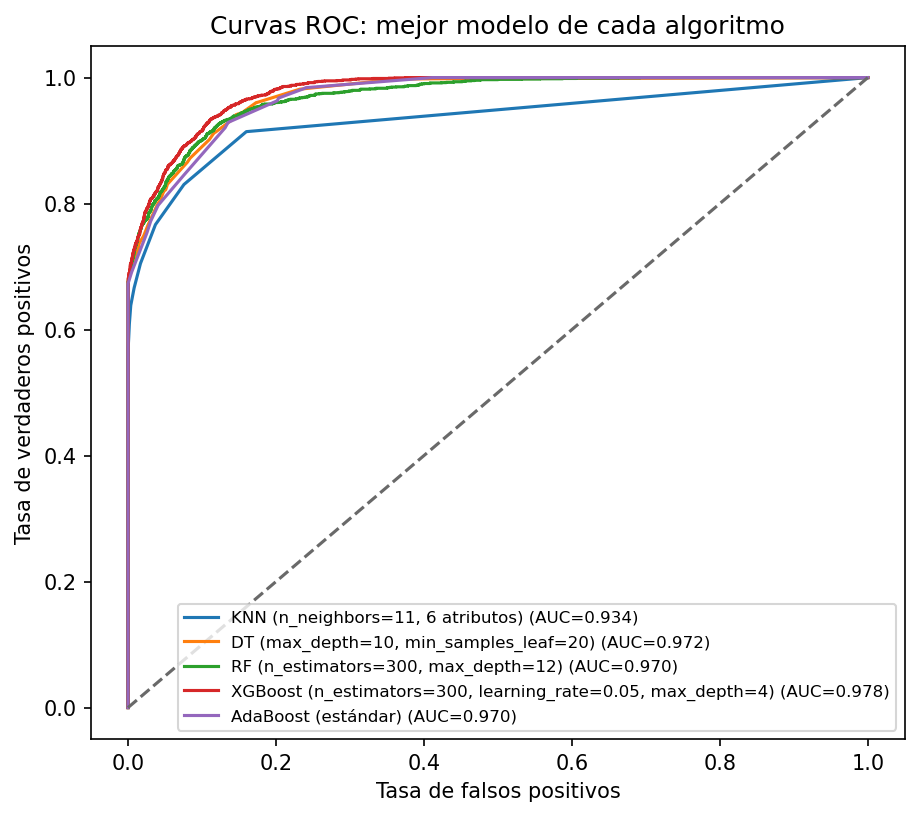
\includegraphics[width=\linewidth]{diabetes/roc_mejores.png}\caption{Curvas ROC}\end{subfigure}
\caption{Comparación de los mejores modelos de diabetes.}
\end{figure}

\begin{figure}[H]
\centering
\begin{subfigure}{0.49\textwidth}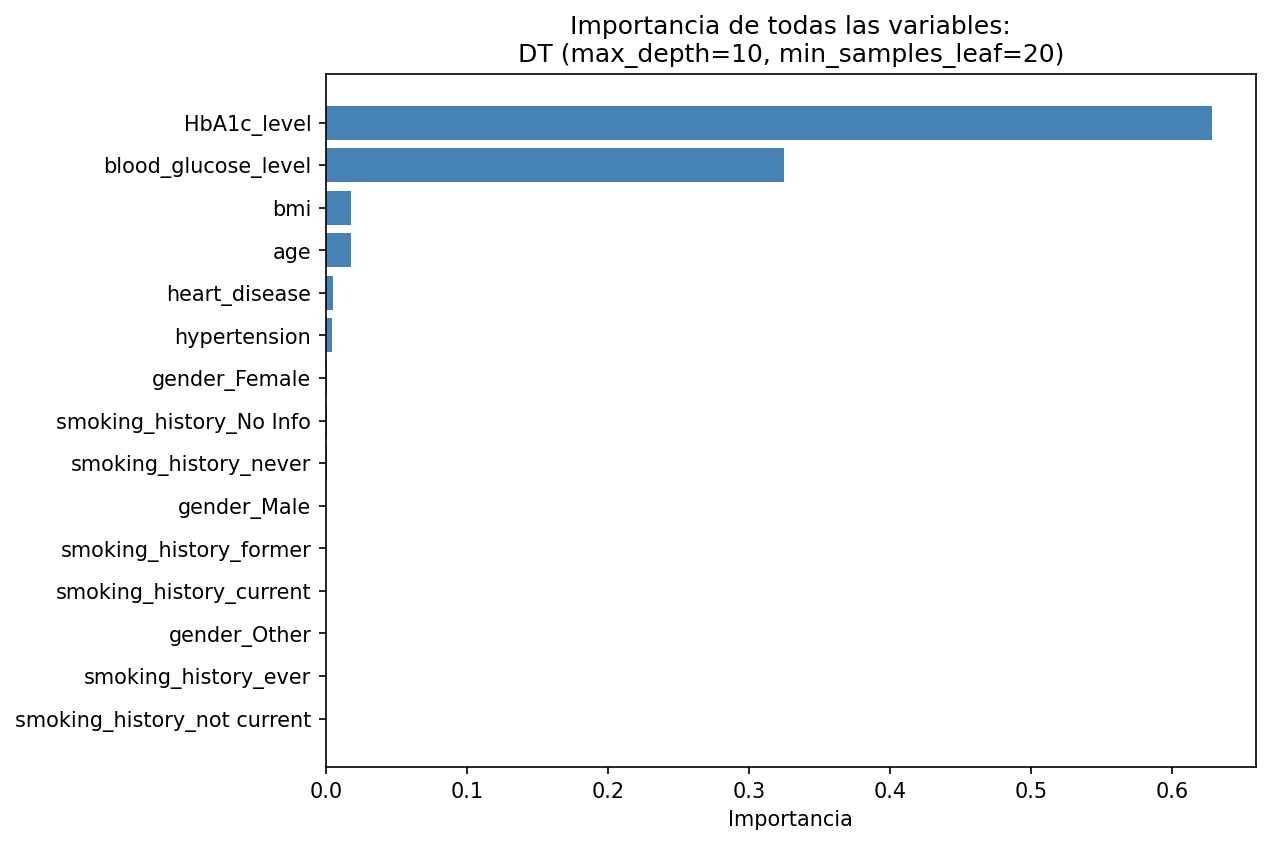
\includegraphics[width=\linewidth]{diabetes/dt_importancia.png}\caption{DT}\end{subfigure}
\begin{subfigure}{0.49\textwidth}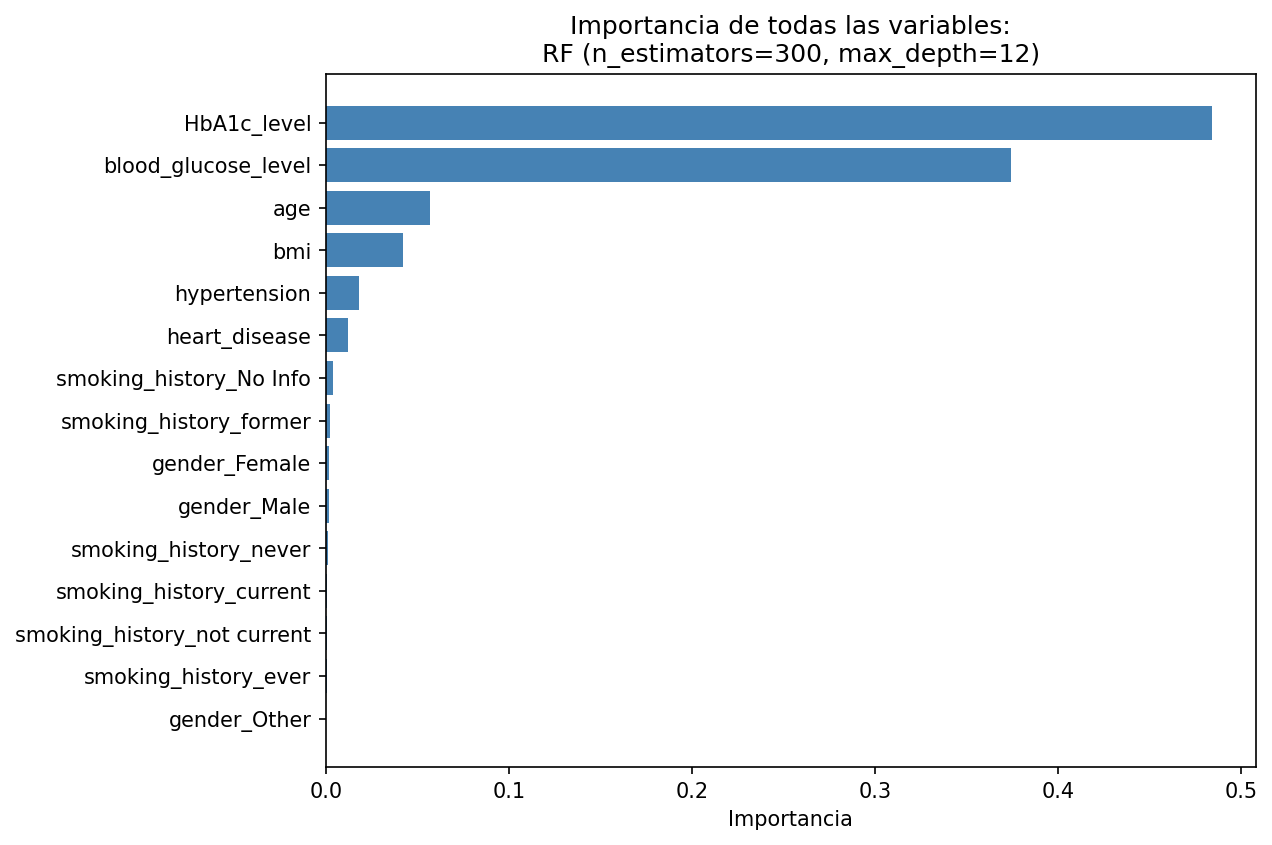
\includegraphics[width=\linewidth]{diabetes/rf_importancia.png}\caption{RF}\end{subfigure}
\begin{subfigure}{0.49\textwidth}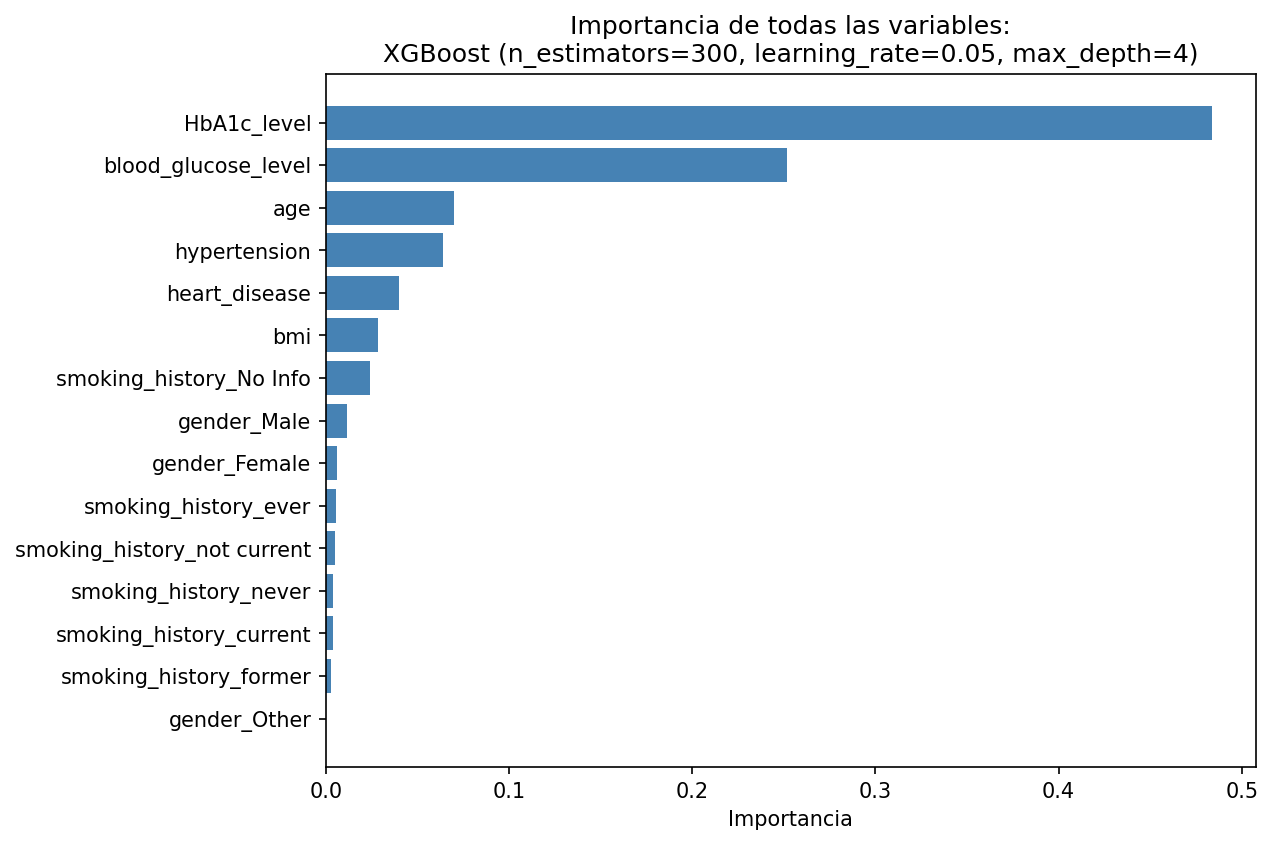
\includegraphics[width=\linewidth]{diabetes/xgboost_importancia.png}\caption{XGBoost}\end{subfigure}
\begin{subfigure}{0.49\textwidth}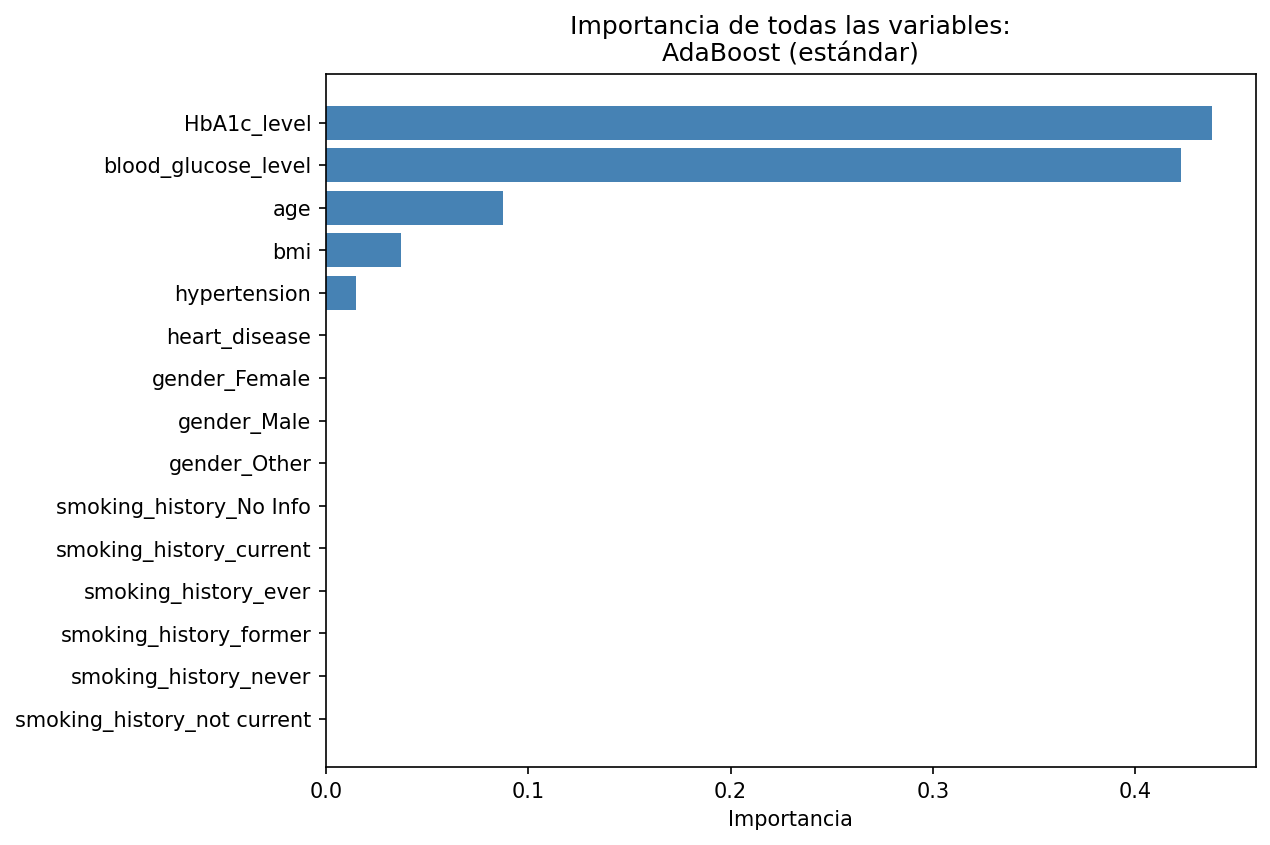
\includegraphics[width=\linewidth]{diabetes/adaboost_importancia.png}\caption{AdaBoost}\end{subfigure}
\caption{Importancia de las 15 variables (después del one-hot) en los mejores modelos de árboles.}
\end{figure}

La importancia de variables confirma lo del análisis exploratorio. HbA1c y glucosa juntas suman entre el 73\,\% (XGBoost) y el 95\,\% (DT) de la importancia, y en ese orden están después la edad, el IMC, la hipertensión y las enfermedades del corazón. Las columnas del one-hot de \texttt{gender} y \texttt{smoking\_history} casi no aportan, y en AdaBoost su importancia es exactamente 0. Esto coincide con lo que dice la \citet{ada2024}: la HbA1c y la glucosa son los criterios de diagnóstico, y la edad y el sobrepeso son factores de riesgo. \textbf{El mejor modelo para diabetes es XGBoost} con 300 árboles, tasa 0.05 y profundidad 4: tiene el F1 macro más alto en la prueba y en la validación cruzada, y la mejor AUC.

% ======================================================================
\section{Conclusiones}

Este laboratorio mostró que el desempeño de un clasificador depende primero de cuánta información tienen los datos sobre la clase y después del algoritmo. En potabilidad, ninguna de las nueve variables tiene una correlación con la clase mayor a 0.034, y ni el mejor modelo, un Random Forest con 500 árboles y pesos \texttt{balanced\_subsample}, pasó de un F1 macro de 0.6047 (0.6205 en validación cruzada) ni de una AUC de 0.68, apenas por encima del clasificador trivial. En diabetes, en cambio, la HbA1c y la glucosa reproducen los criterios de diagnóstico de la \citet{ada2024}: cuatro de los cinco algoritmos llegaron a un F1 macro de 0.89 y una AUC mayor a 0.97, y los modelos de árboles detectaron prácticamente el 67\,\% de diabéticos que los umbrales identifican con total seguridad, pero ninguno logró separar bien el tercio restante, donde las clases se traslapan, lo que confirma que el límite lo ponen los datos y no el modelo \citep{he2009}. También vimos que la configuración estándar casi nunca fue la mejor: el árbol sin límite memorizó el entrenamiento en los dos datasets (478 y 3313 hojas) y quedó entre los peores, y limitar su profundidad lo mejoró mucho, tal como plantean \citet{breiman1984}; los ensambles fueron más estables que un solo árbol, como esperábamos por \citet{breiman2001}; y el \textit{boosting} solo funcionó cuando su clasificador base podía representar la estructura de los datos, porque los \textit{stumps} de AdaBoost reprodujeron perfectamente la regla de los umbrales en diabetes, pero en potabilidad solo detectaron el 8\,\% de las muestras potables \citep{freund1997}. El preprocesamiento también fue decisivo y depende de cada algoritmo: KNN es inútil sin escalar, y la selección de atributos con ANOVA ayudó en diabetes porque eliminó las columnas del one-hot que distorsionaban las distancias, pero empeoró los modelos en potabilidad porque ninguna variable tiene una diferencia de medias que permita ordenarlas \citep{guyon2003}. Usar el F1 macro como criterio, en vez de la precisión global, fue necesario: con la PG habríamos escogido modelos que casi nunca predicen la clase minoritaria, como KNN con $k=25$ en potabilidad, y la comparación de las curvas ROC mostró que dar más peso a la clase positiva (\texttt{class\_weight} o \texttt{scale\_pos\_weight}) no cambia la AUC sino solo el umbral, es decir, cambia cuántos falsos positivos se aceptan para detectar más positivos, y esa decisión depende del costo de cada error en la aplicación \citep{fawcett2006,sokolova2009}. Por último, la validación cruzada mostró que en diabetes las diferencias entre XGBoost, DT, RF y AdaBoost son menores que su variabilidad, por lo que escogimos XGBoost por su AUC más alta y no por el F1, mientras que en potabilidad confirmó a Random Forest como el modelo más sólido \citep{kohavi1995}; en ambos casos, el uso del framework con el preprocesamiento dentro del \texttt{Pipeline}, una semilla fija y el historial de experimentos permitió que todos los resultados se puedan reproducir y comparar en las mismas condiciones \citep{pedregosa2011}.

% ======================================================================
\begin{thebibliography}{99}

\bibitem[{American Diabetes Association Professional Practice Committee}(2024)]{ada2024}
American Diabetes Association Professional Practice Committee (2024). 2. Diagnosis and classification of diabetes: Standards of Care in Diabetes---2024. \textit{Diabetes Care}, 47(Suppl.~1), S20--S42.

\bibitem[Breiman(1996)]{breiman1996}
Breiman, L. (1996). Bagging predictors. \textit{Machine Learning}, 24(2), 123--140.

\bibitem[Breiman(2001)]{breiman2001}
Breiman, L. (2001). Random forests. \textit{Machine Learning}, 45(1), 5--32.

\bibitem[Breiman et~al.(1984)]{breiman1984}
Breiman, L., Friedman, J. H., Olshen, R. A. y Stone, C. J. (1984). \textit{Classification and Regression Trees}. Wadsworth.

\bibitem[Chen y Guestrin(2016)]{chen2016}
Chen, T. y Guestrin, C. (2016). XGBoost: A scalable tree boosting system. En \textit{Proceedings of the 22nd ACM SIGKDD International Conference on Knowledge Discovery and Data Mining}, 785--794.

\bibitem[Cover y Hart(1967)]{cover1967}
Cover, T. y Hart, P. (1967). Nearest neighbor pattern classification. \textit{IEEE Transactions on Information Theory}, 13(1), 21--27.

\bibitem[Fawcett(2006)]{fawcett2006}
Fawcett, T. (2006). An introduction to ROC analysis. \textit{Pattern Recognition Letters}, 27(8), 861--874.

\bibitem[Freund y Schapire(1997)]{freund1997}
Freund, Y. y Schapire, R. E. (1997). A decision-theoretic generalization of on-line learning and an application to boosting. \textit{Journal of Computer and System Sciences}, 55(1), 119--139.

\bibitem[Friedman(2001)]{friedman2001}
Friedman, J. H. (2001). Greedy function approximation: A gradient boosting machine. \textit{The Annals of Statistics}, 29(5), 1189--1232.

\bibitem[Guyon y Elisseeff(2003)]{guyon2003}
Guyon, I. y Elisseeff, A. (2003). An introduction to variable and feature selection. \textit{Journal of Machine Learning Research}, 3, 1157--1182.

\bibitem[Hastie et~al.(2009)]{hastie2009}
Hastie, T., Tibshirani, R. y Friedman, J. (2009). \textit{The Elements of Statistical Learning: Data Mining, Inference, and Prediction} (2.\textsuperscript{a} ed.). Springer.

\bibitem[He y Garcia(2009)]{he2009}
He, H. y Garcia, E. A. (2009). Learning from imbalanced data. \textit{IEEE Transactions on Knowledge and Data Engineering}, 21(9), 1263--1284.

\bibitem[James et~al.(2013)]{james2013}
James, G., Witten, D., Hastie, T. y Tibshirani, R. (2013). \textit{An Introduction to Statistical Learning with Applications in R}. Springer.

\bibitem[Kadiwal(2021)]{kadiwal2021}
Kadiwal, A. (2021). \textit{Water Quality} [conjunto de datos]. Kaggle. \url{https://www.kaggle.com/datasets/adityakadiwal/water-potability}

\bibitem[Kohavi(1995)]{kohavi1995}
Kohavi, R. (1995). A study of cross-validation and bootstrap for accuracy estimation and model selection. En \textit{Proceedings of the 14th International Joint Conference on Artificial Intelligence}, vol. 2, 1137--1145.

\bibitem[Mustafa(2023)]{mustafa2023}
Mustafa, M. (2023). \textit{Diabetes prediction dataset} [conjunto de datos]. Kaggle. \url{https://www.kaggle.com/datasets/iammustafatz/diabetes-prediction-dataset}

\bibitem[Pedregosa et~al.(2011)]{pedregosa2011}
Pedregosa, F., Varoquaux, G., Gramfort, A., Michel, V., Thirion, B., Grisel, O. et~al. (2011). Scikit-learn: Machine learning in Python. \textit{Journal of Machine Learning Research}, 12, 2825--2830.

\bibitem[Quinlan(1986)]{quinlan1986}
Quinlan, J. R. (1986). Induction of decision trees. \textit{Machine Learning}, 1(1), 81--106.

\bibitem[Sokolova y Lapalme(2009)]{sokolova2009}
Sokolova, M. y Lapalme, G. (2009). A systematic analysis of performance measures for classification tasks. \textit{Information Processing \& Management}, 45(4), 427--437.

\bibitem[Tukey(1977)]{tukey1977}
Tukey, J. W. (1977). \textit{Exploratory Data Analysis}. Addison-Wesley.

\bibitem[{World Health Organization}(2022)]{who2022}
World Health Organization (2022). \textit{Guidelines for Drinking-water Quality: Fourth Edition Incorporating the First and Second Addenda}. WHO.

\end{thebibliography}

\end{document}
